% -*- program: pdflatex -*-

\documentclass[11pt]{article}
\usepackage{evolution}
\usepackage[section]{placeins}
\usepackage{geometry}
\usepackage{rotating}
 \usepackage{soul}
 \usepackage{grffile} %necessary to have dots in filenames that are not extensions

\begin{document}


\section*{Supplemental information}
\bigskip

\clearpage

%
% FIGURES
%


%Fig S1: Gene 2 tree
\begin{suppfigure}
\centering
\caption{
RdRp gene tree with bootstrap values.
}
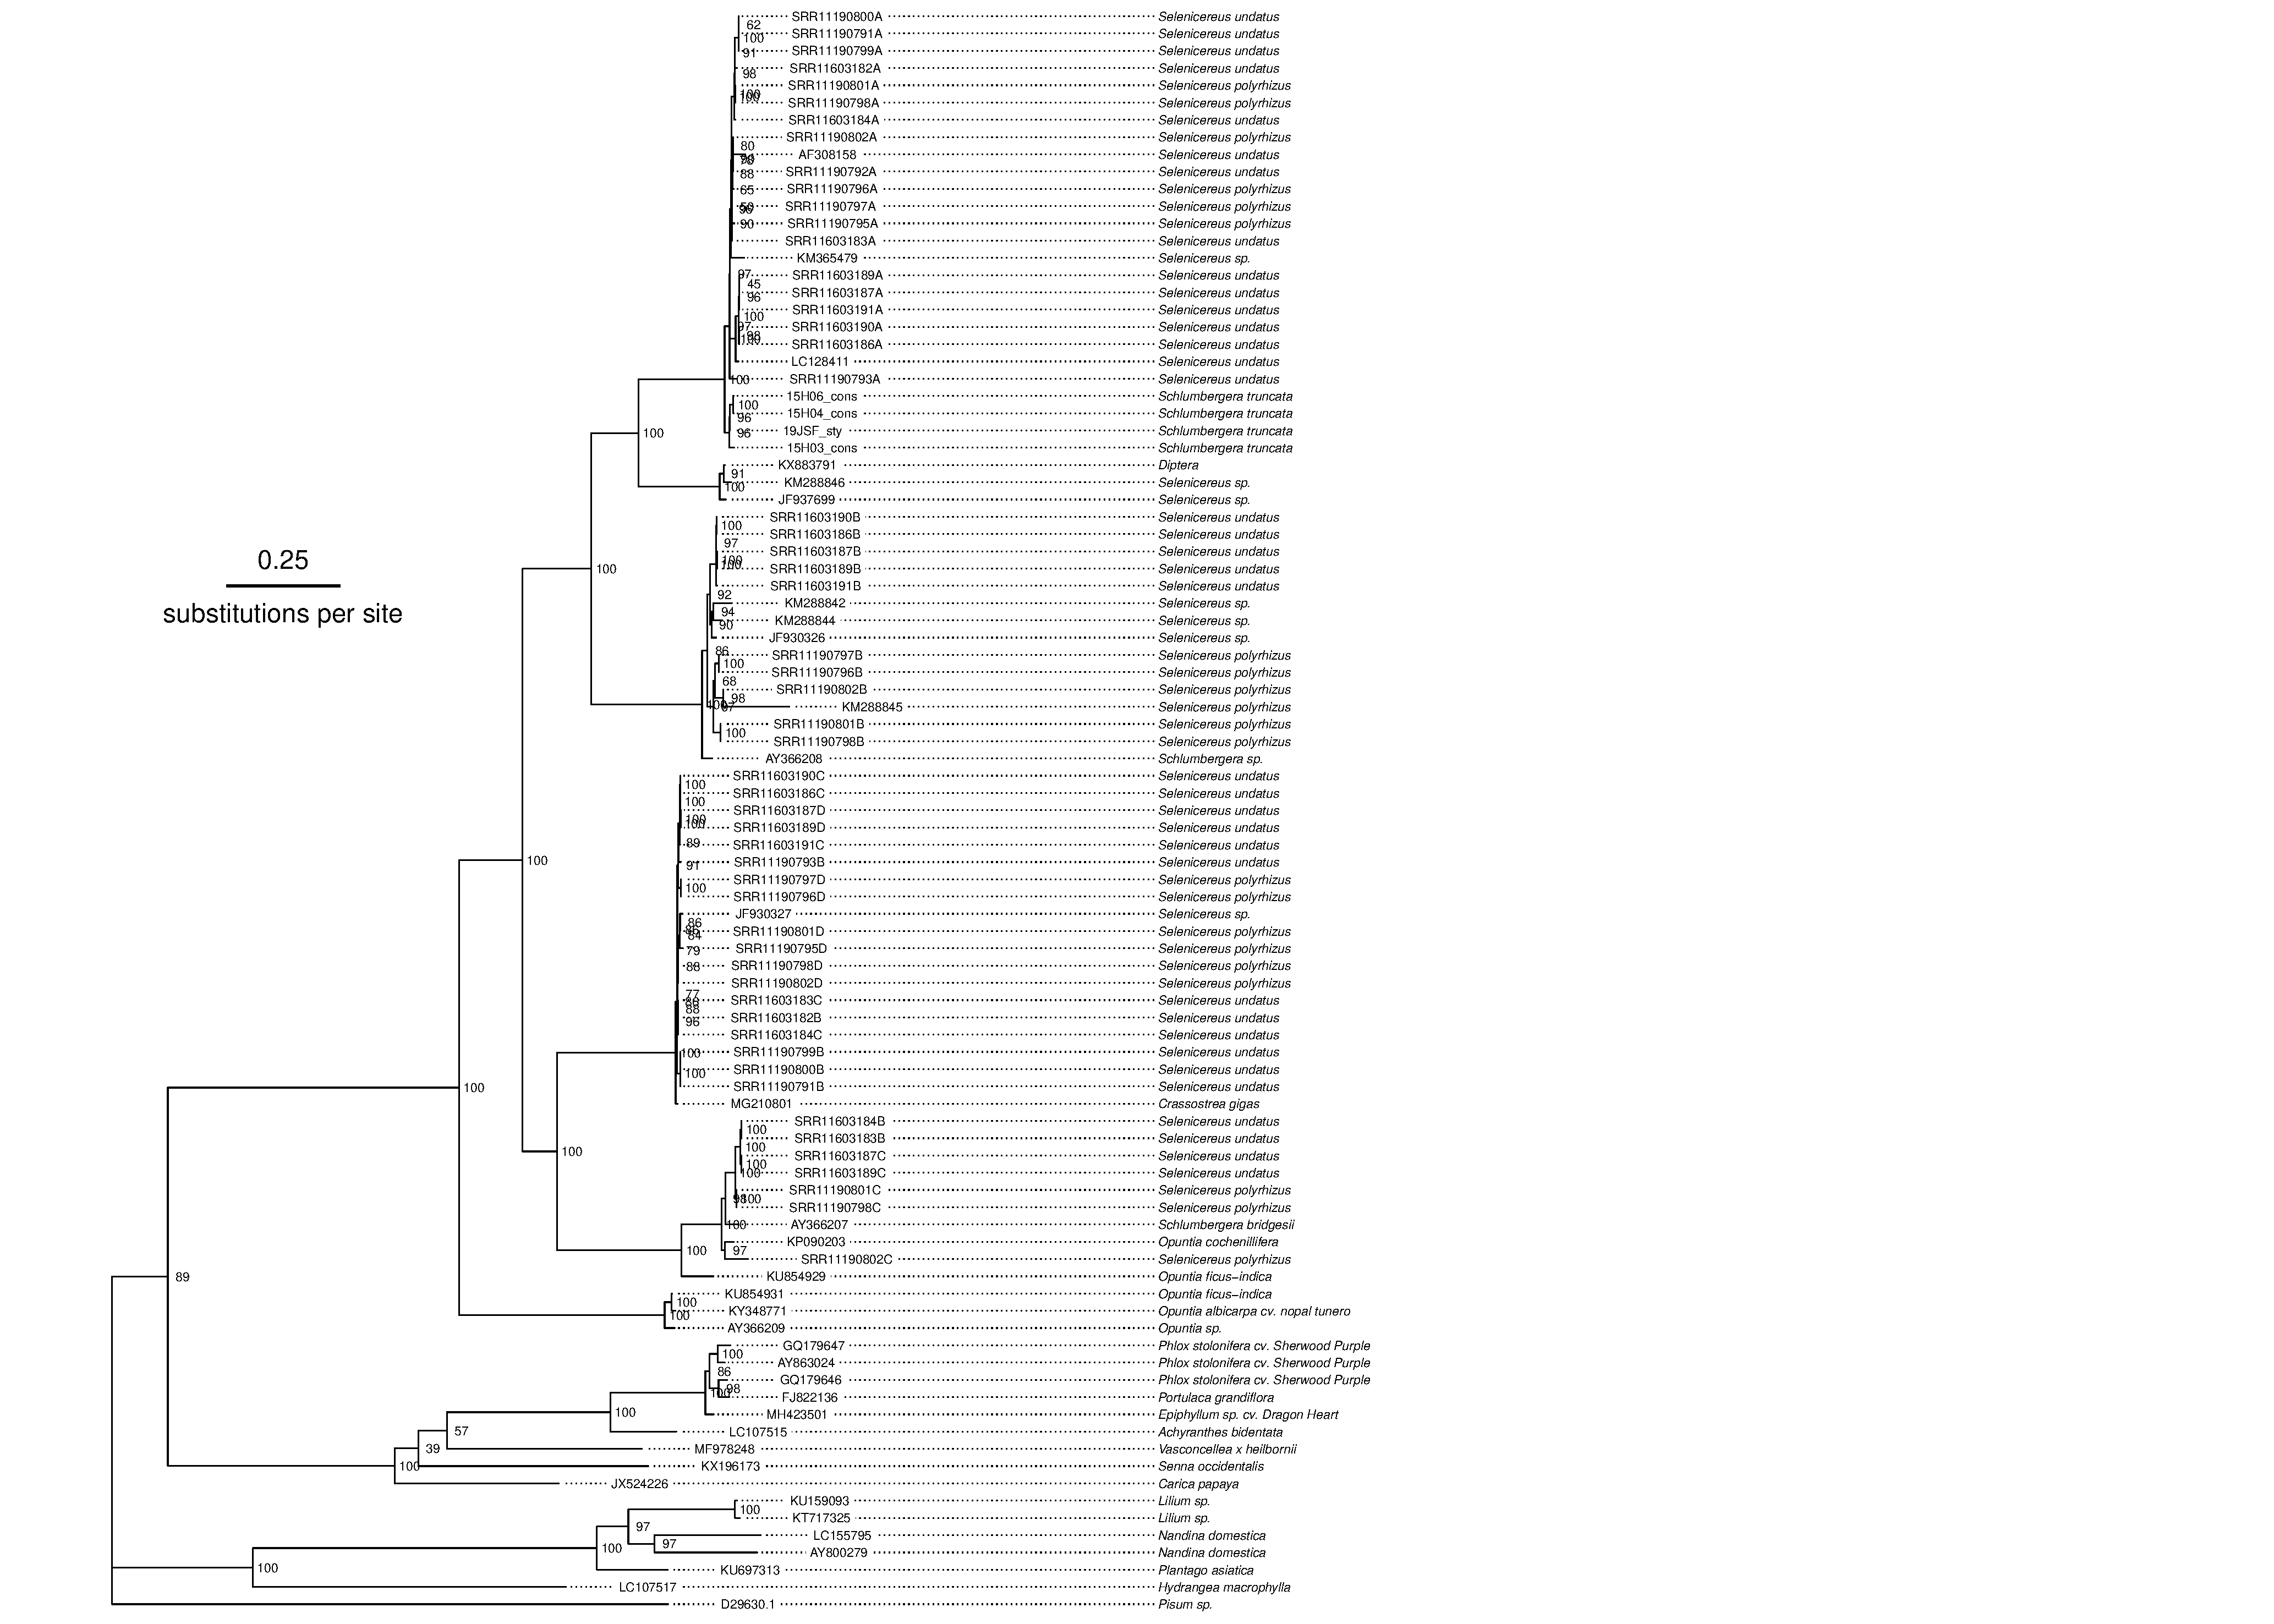
\includegraphics[width=1.5\textwidth]{supplementaryinfo/rdrp_tr.pdf}
\label{fig:genetree1}
\end{suppfigure}
\clearpage


%Fig S2: Gene 2 tree
\begin{suppfigure}
\centering
\caption{
TGB1 gene tree with bootstrap values constructed with the same method as Figure S1.
}
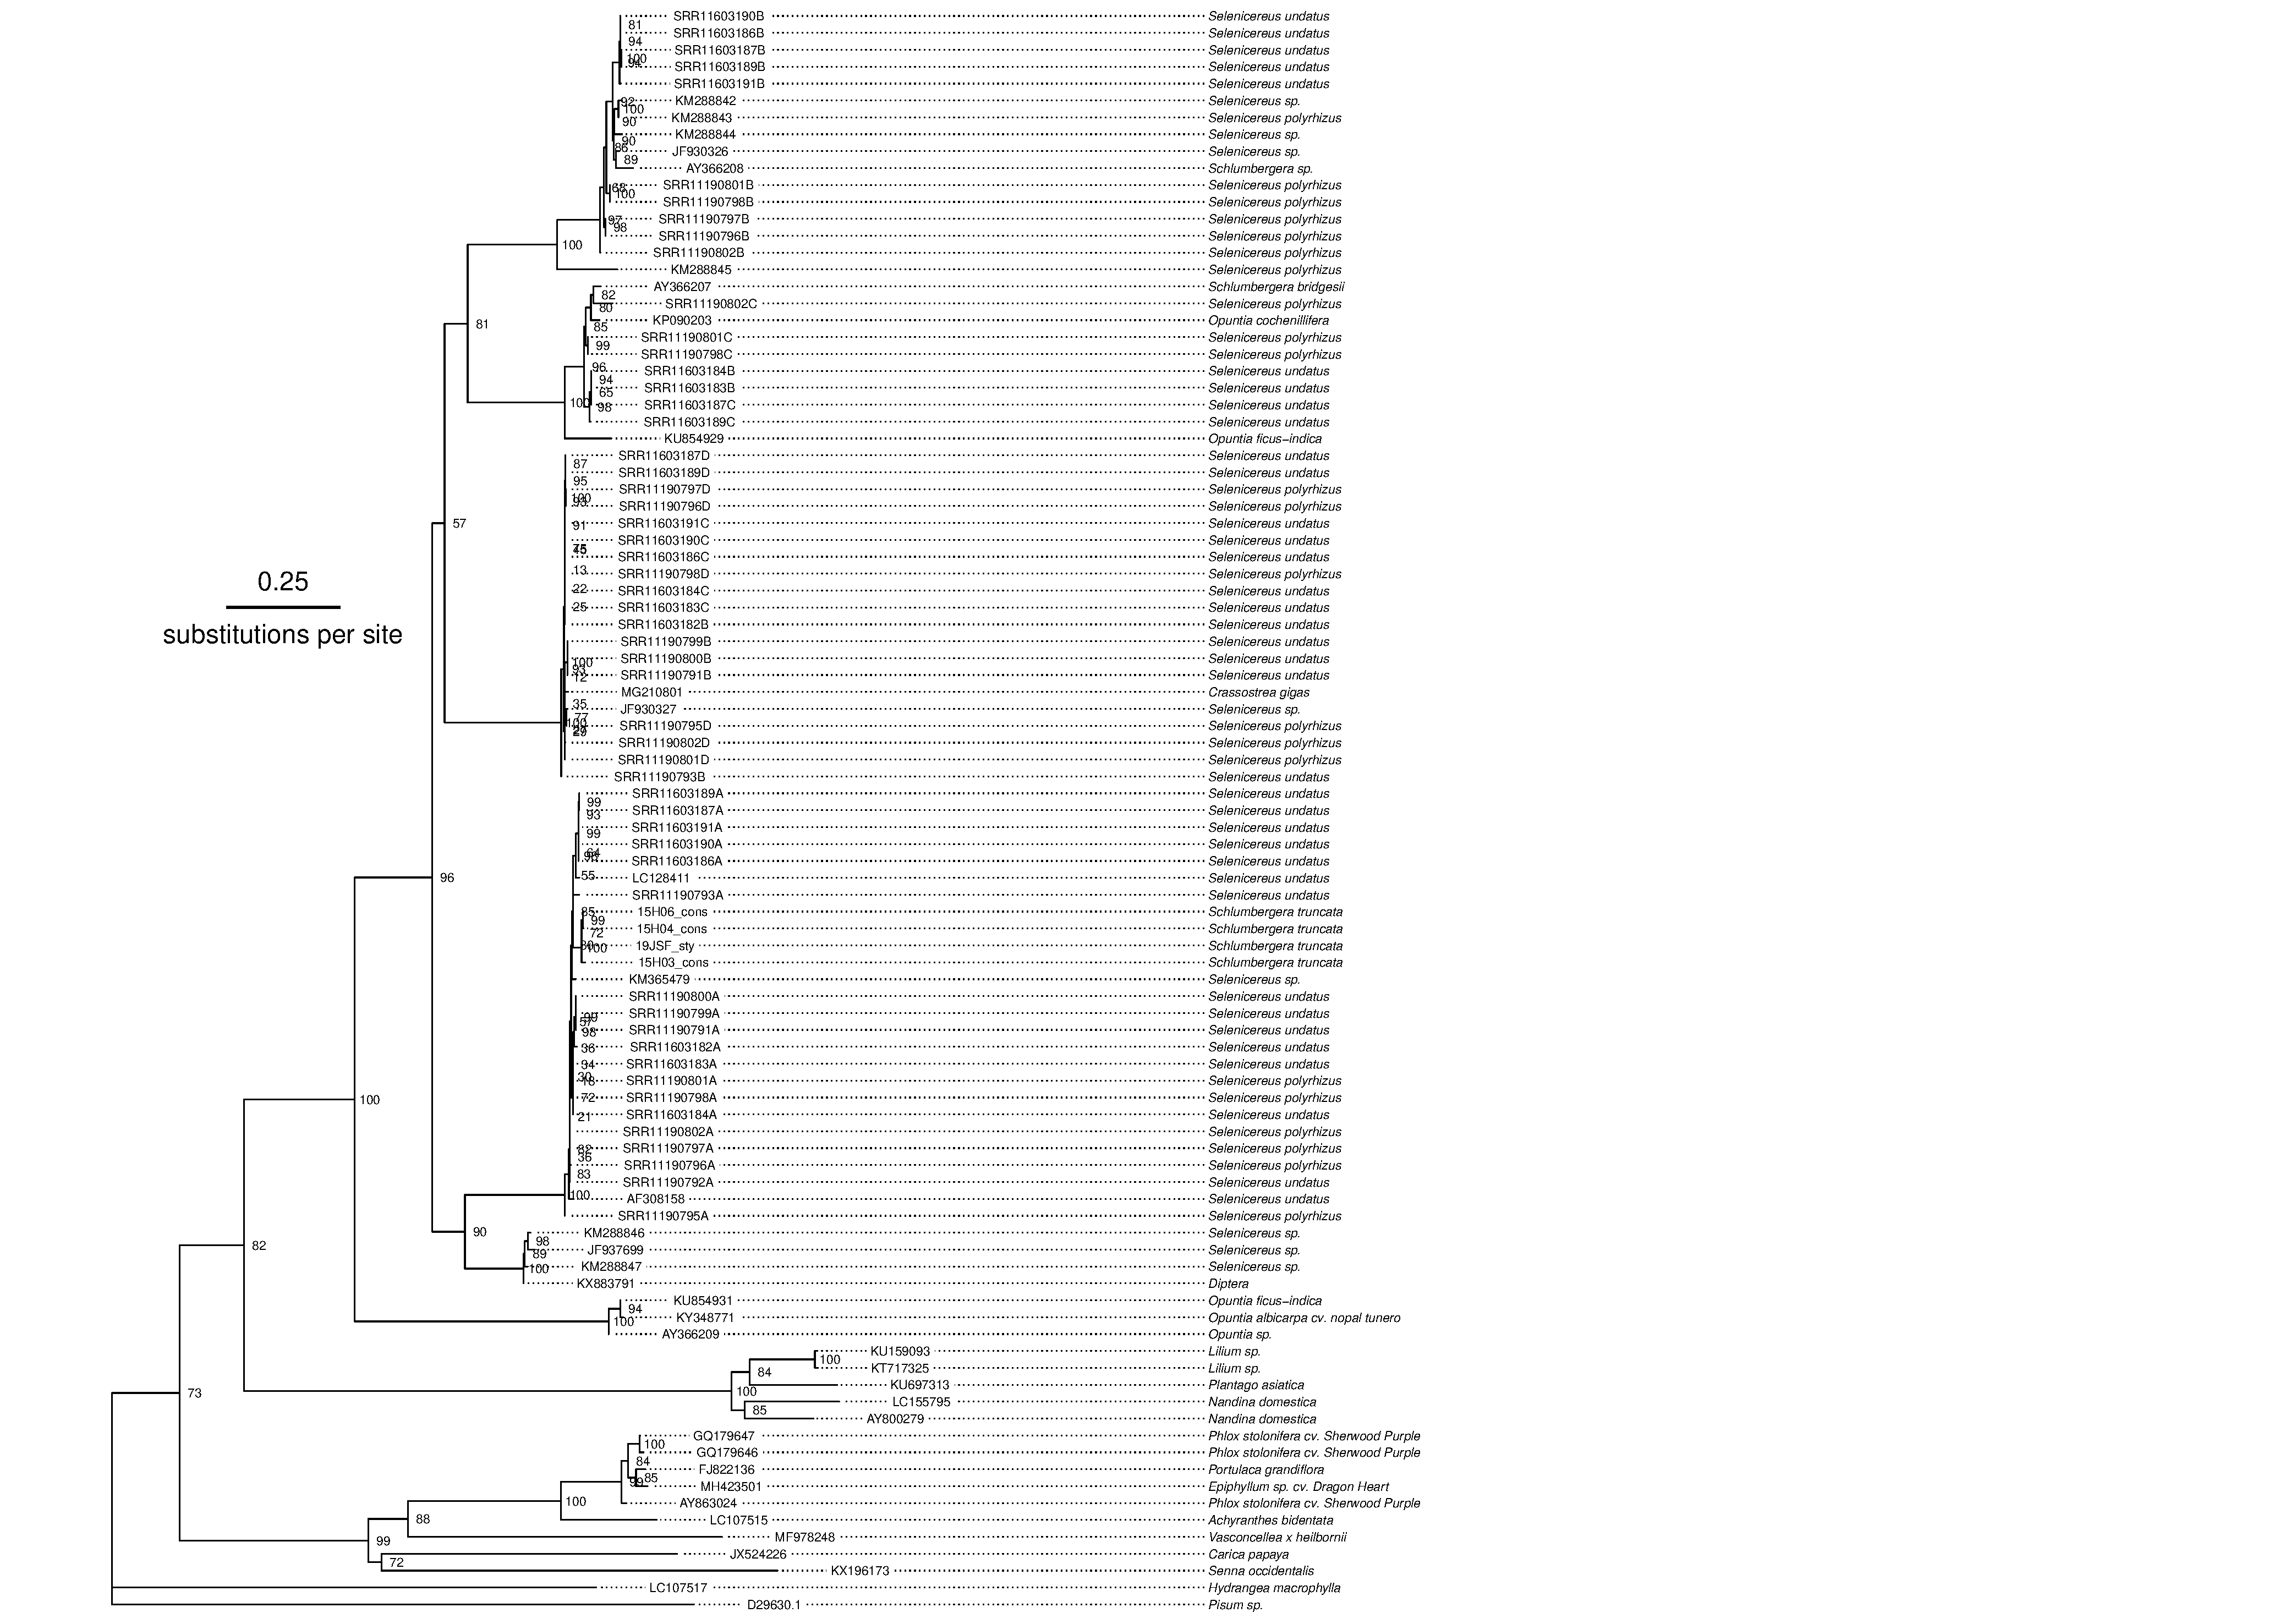
\includegraphics[width=1.5\textwidth]{supplementaryinfo/tgb1_tr.pdf}
\label{fig:genetree2}
\end{suppfigure}
\clearpage

%Fig S3: Gene 3 tree
\begin{suppfigure}
\centering
\caption{
TGB2 gene tree with bootstrap values constructed with the same method as Figure S1.
}
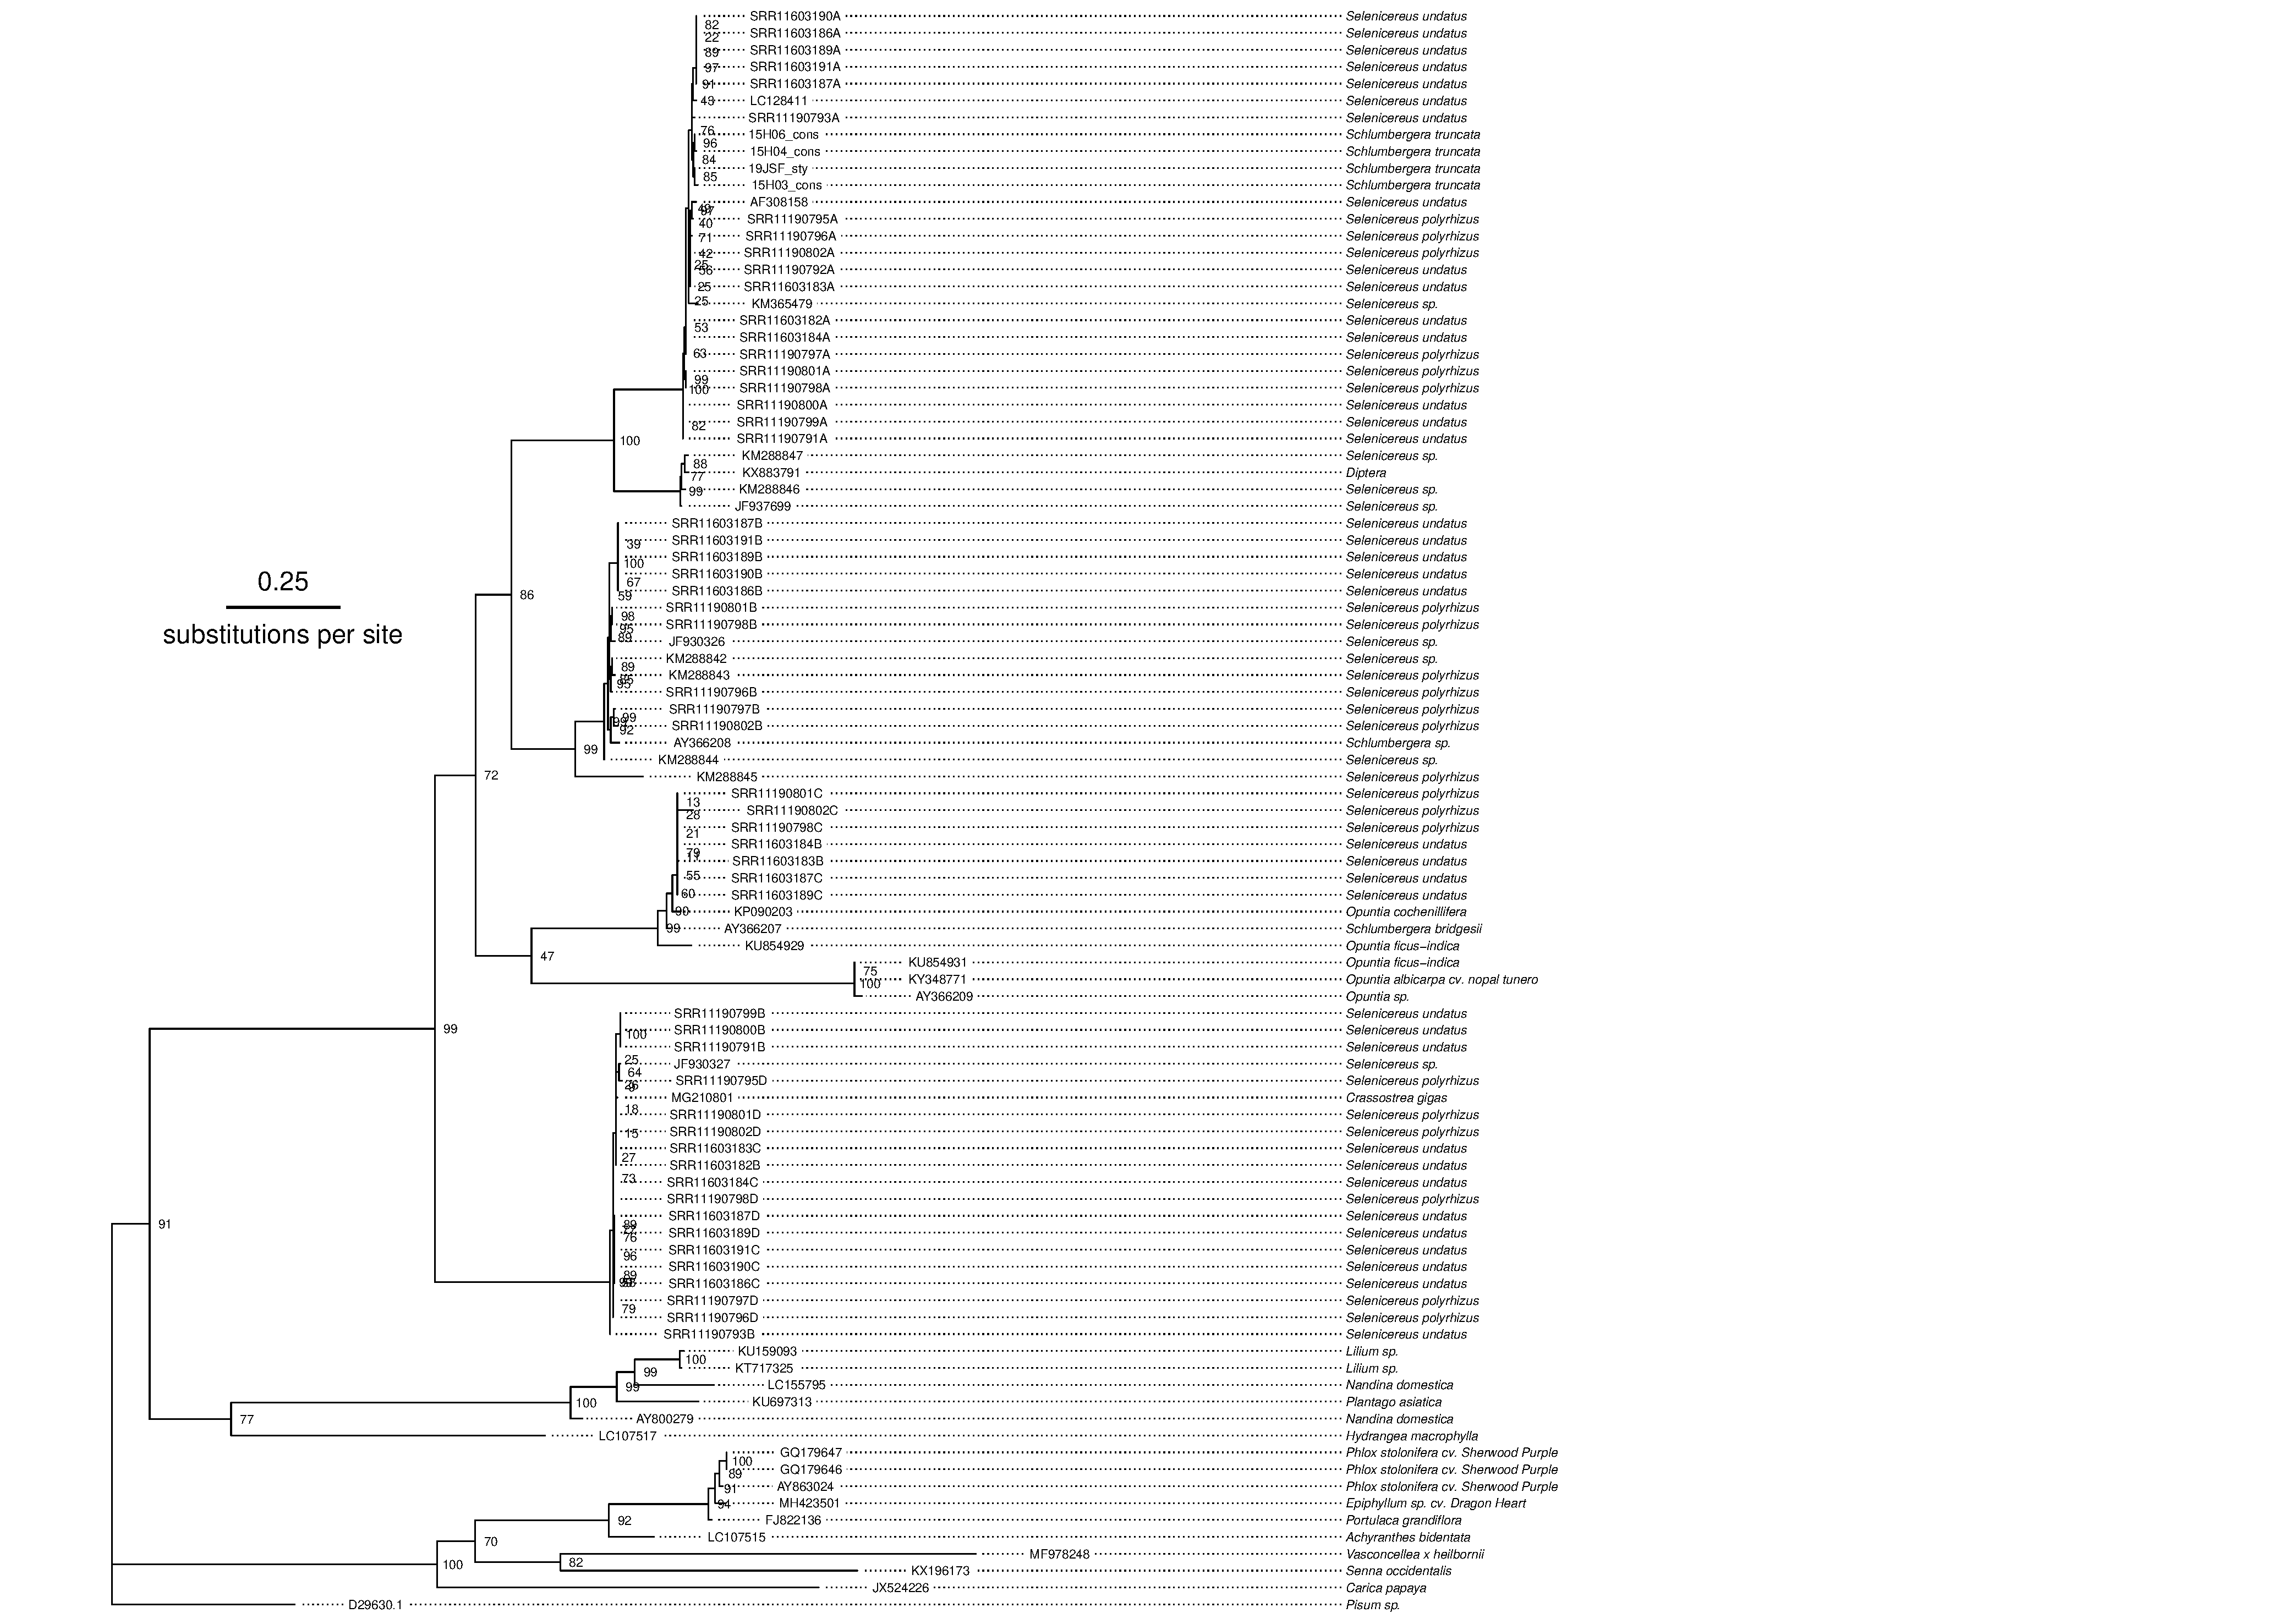
\includegraphics[width=1.5\textwidth]{supplementaryinfo/tgb2_tr.pdf}
\label{fig:genetree3}
\end{suppfigure}
\clearpage

%Fig S4: Gene 4 tree
\begin{suppfigure}
\centering
\caption{
TGB3 gene tree with bootstrap values constructed with the same method as Figure S1.
}
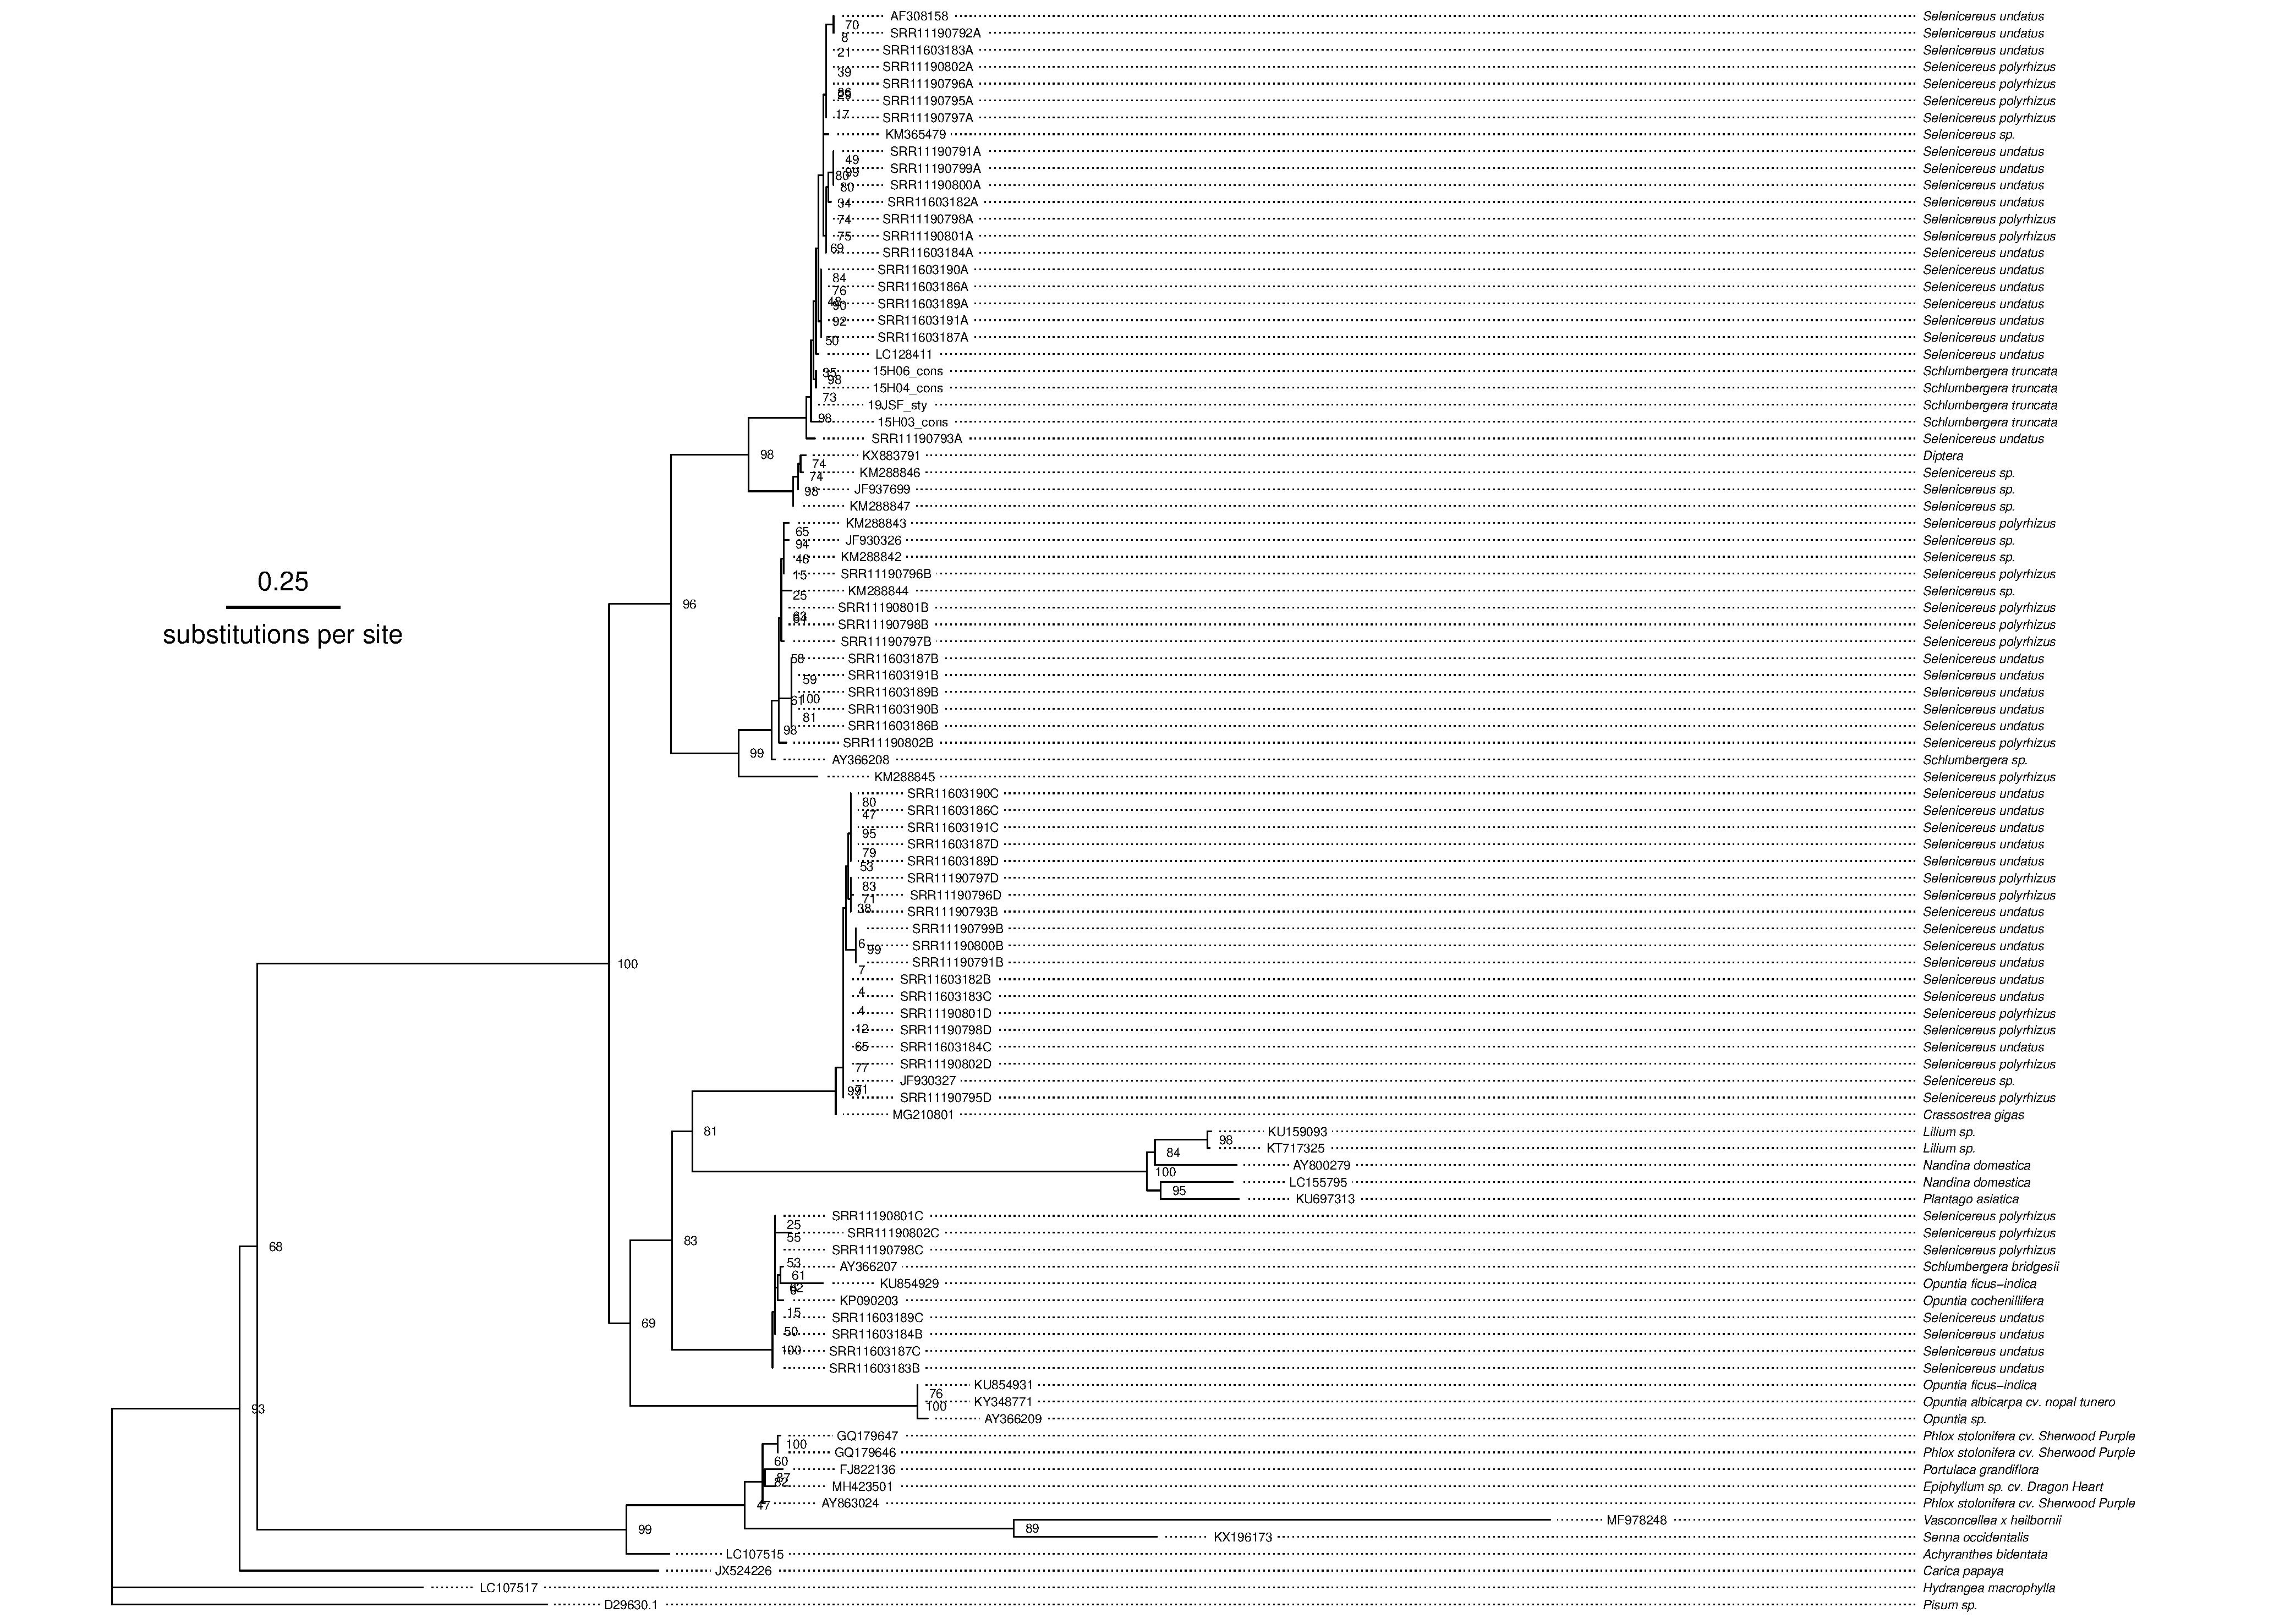
\includegraphics[width=1.2\textwidth]{supplementaryinfo/tgb3_tr.pdf}
\label{fig:genetree4}
\end{suppfigure}
\clearpage

%Fig S5: Gene 5 tree
\begin{suppfigure}
\centering
\caption{
CP gene tree with bootstrap values constructed with the same method as Figure S1.
}
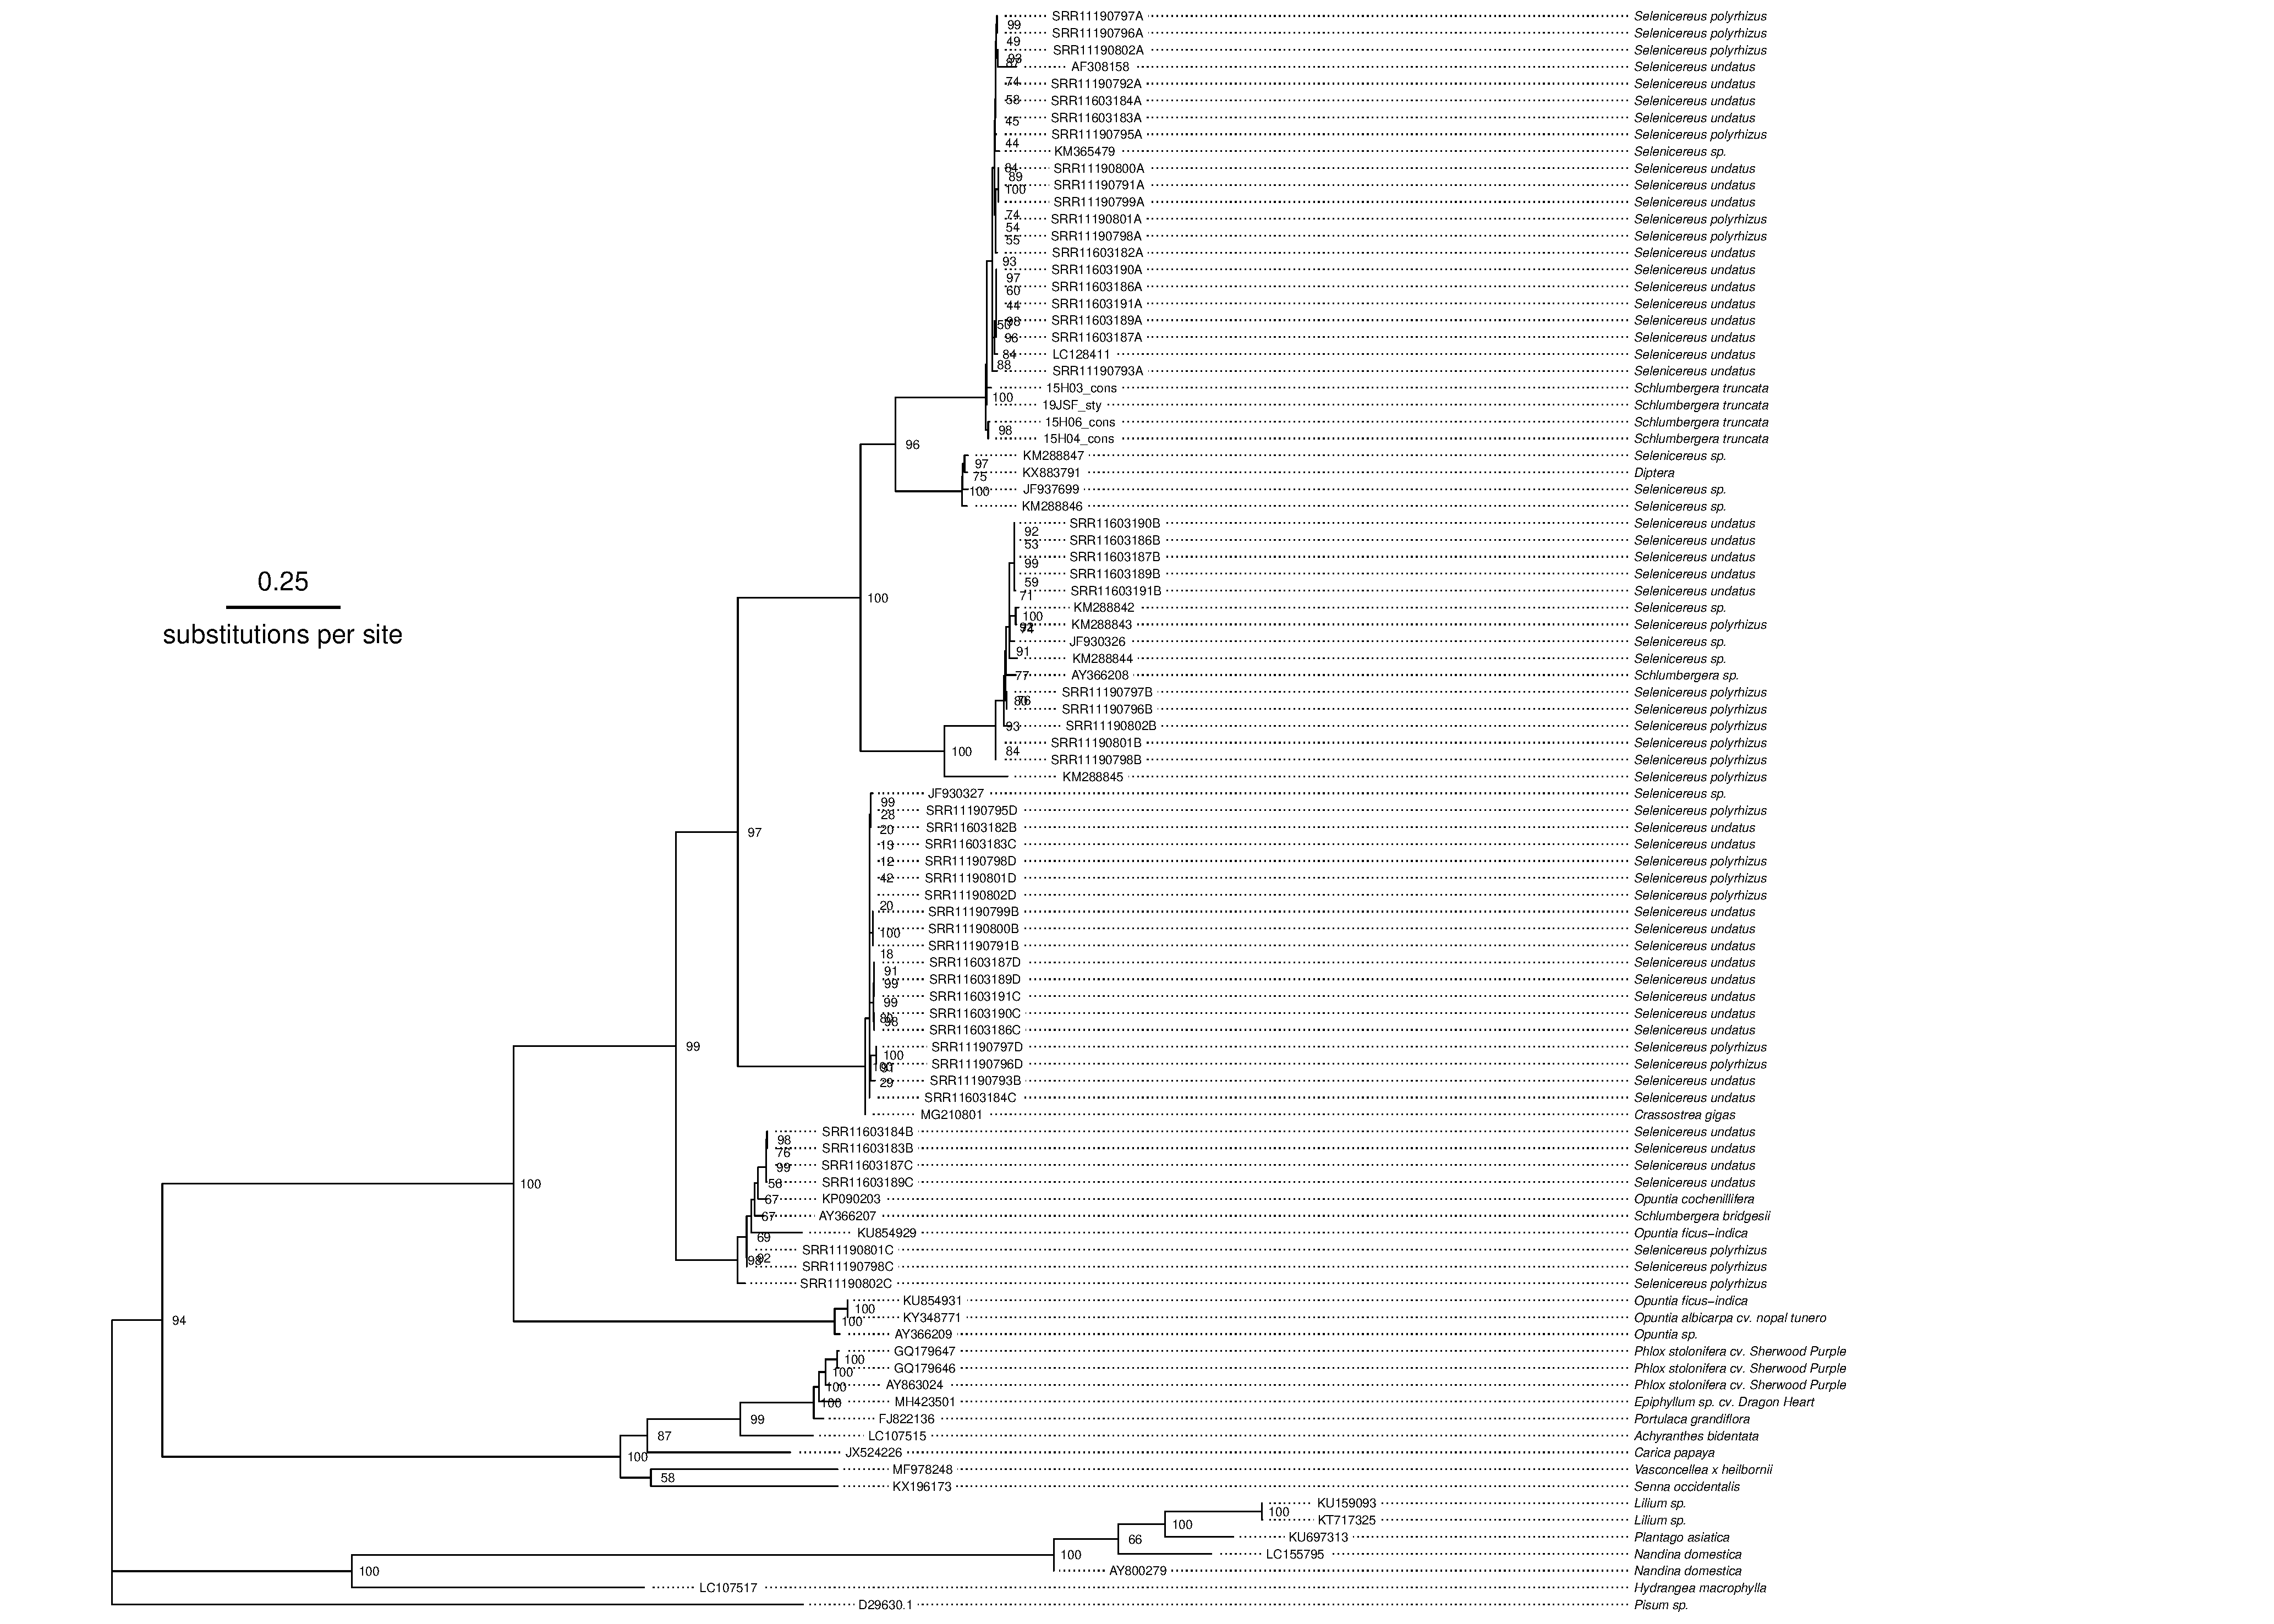
\includegraphics[width=1.3\textwidth]{supplementaryinfo/cp_tr.pdf}
\label{fig:genetree5}
\end{suppfigure}
\clearpage

%Fig S6: Summary of cophylo plots
\begin{suppfigure}
\centering
\caption{
A summary of cophylogenetic comparisons of gene trees (Figures S2-S5) generated using the phytools package in R. Tree topologies largely do not vary between ORF and full sequence.
}
\includegraphics[width=1\textwidth]{supplementaryinfo/cophylo_sum.pdf}
\label{fig:cophylosum}
\end{suppfigure}
\clearpage

%The support values are posterior probabilities of the respective
%delimitations, that is that the split defined by the respective branch
%splits the tree into two distinct species.
%
%The Bayesian version samples alternative delimitations.
%
%So the blue and red colors show you the most plausible delimitation into
%species and individuals from the same species.

%Fig S7:  mPTP tree
\begin{suppfigure}
\centering
\caption{
%TODO
%I am not sure that this is sufficiently clear to an average reviewer or reader. (Both this and the previous figure.) Maybe including this nearer to a color-coded delimitation figure or pointing the reader there would clarify better. Moreover, the description from S6 is slightly better. Also, the posteriors are very hard to see.Someone will complain about that. mPTP whole genome tree with delimitation represented by green and red coloration. Green branches represent delimitation outside of clades and red branches represent delimitation inside of clades.
%Possibly combine these two?; Clarify coloration
}
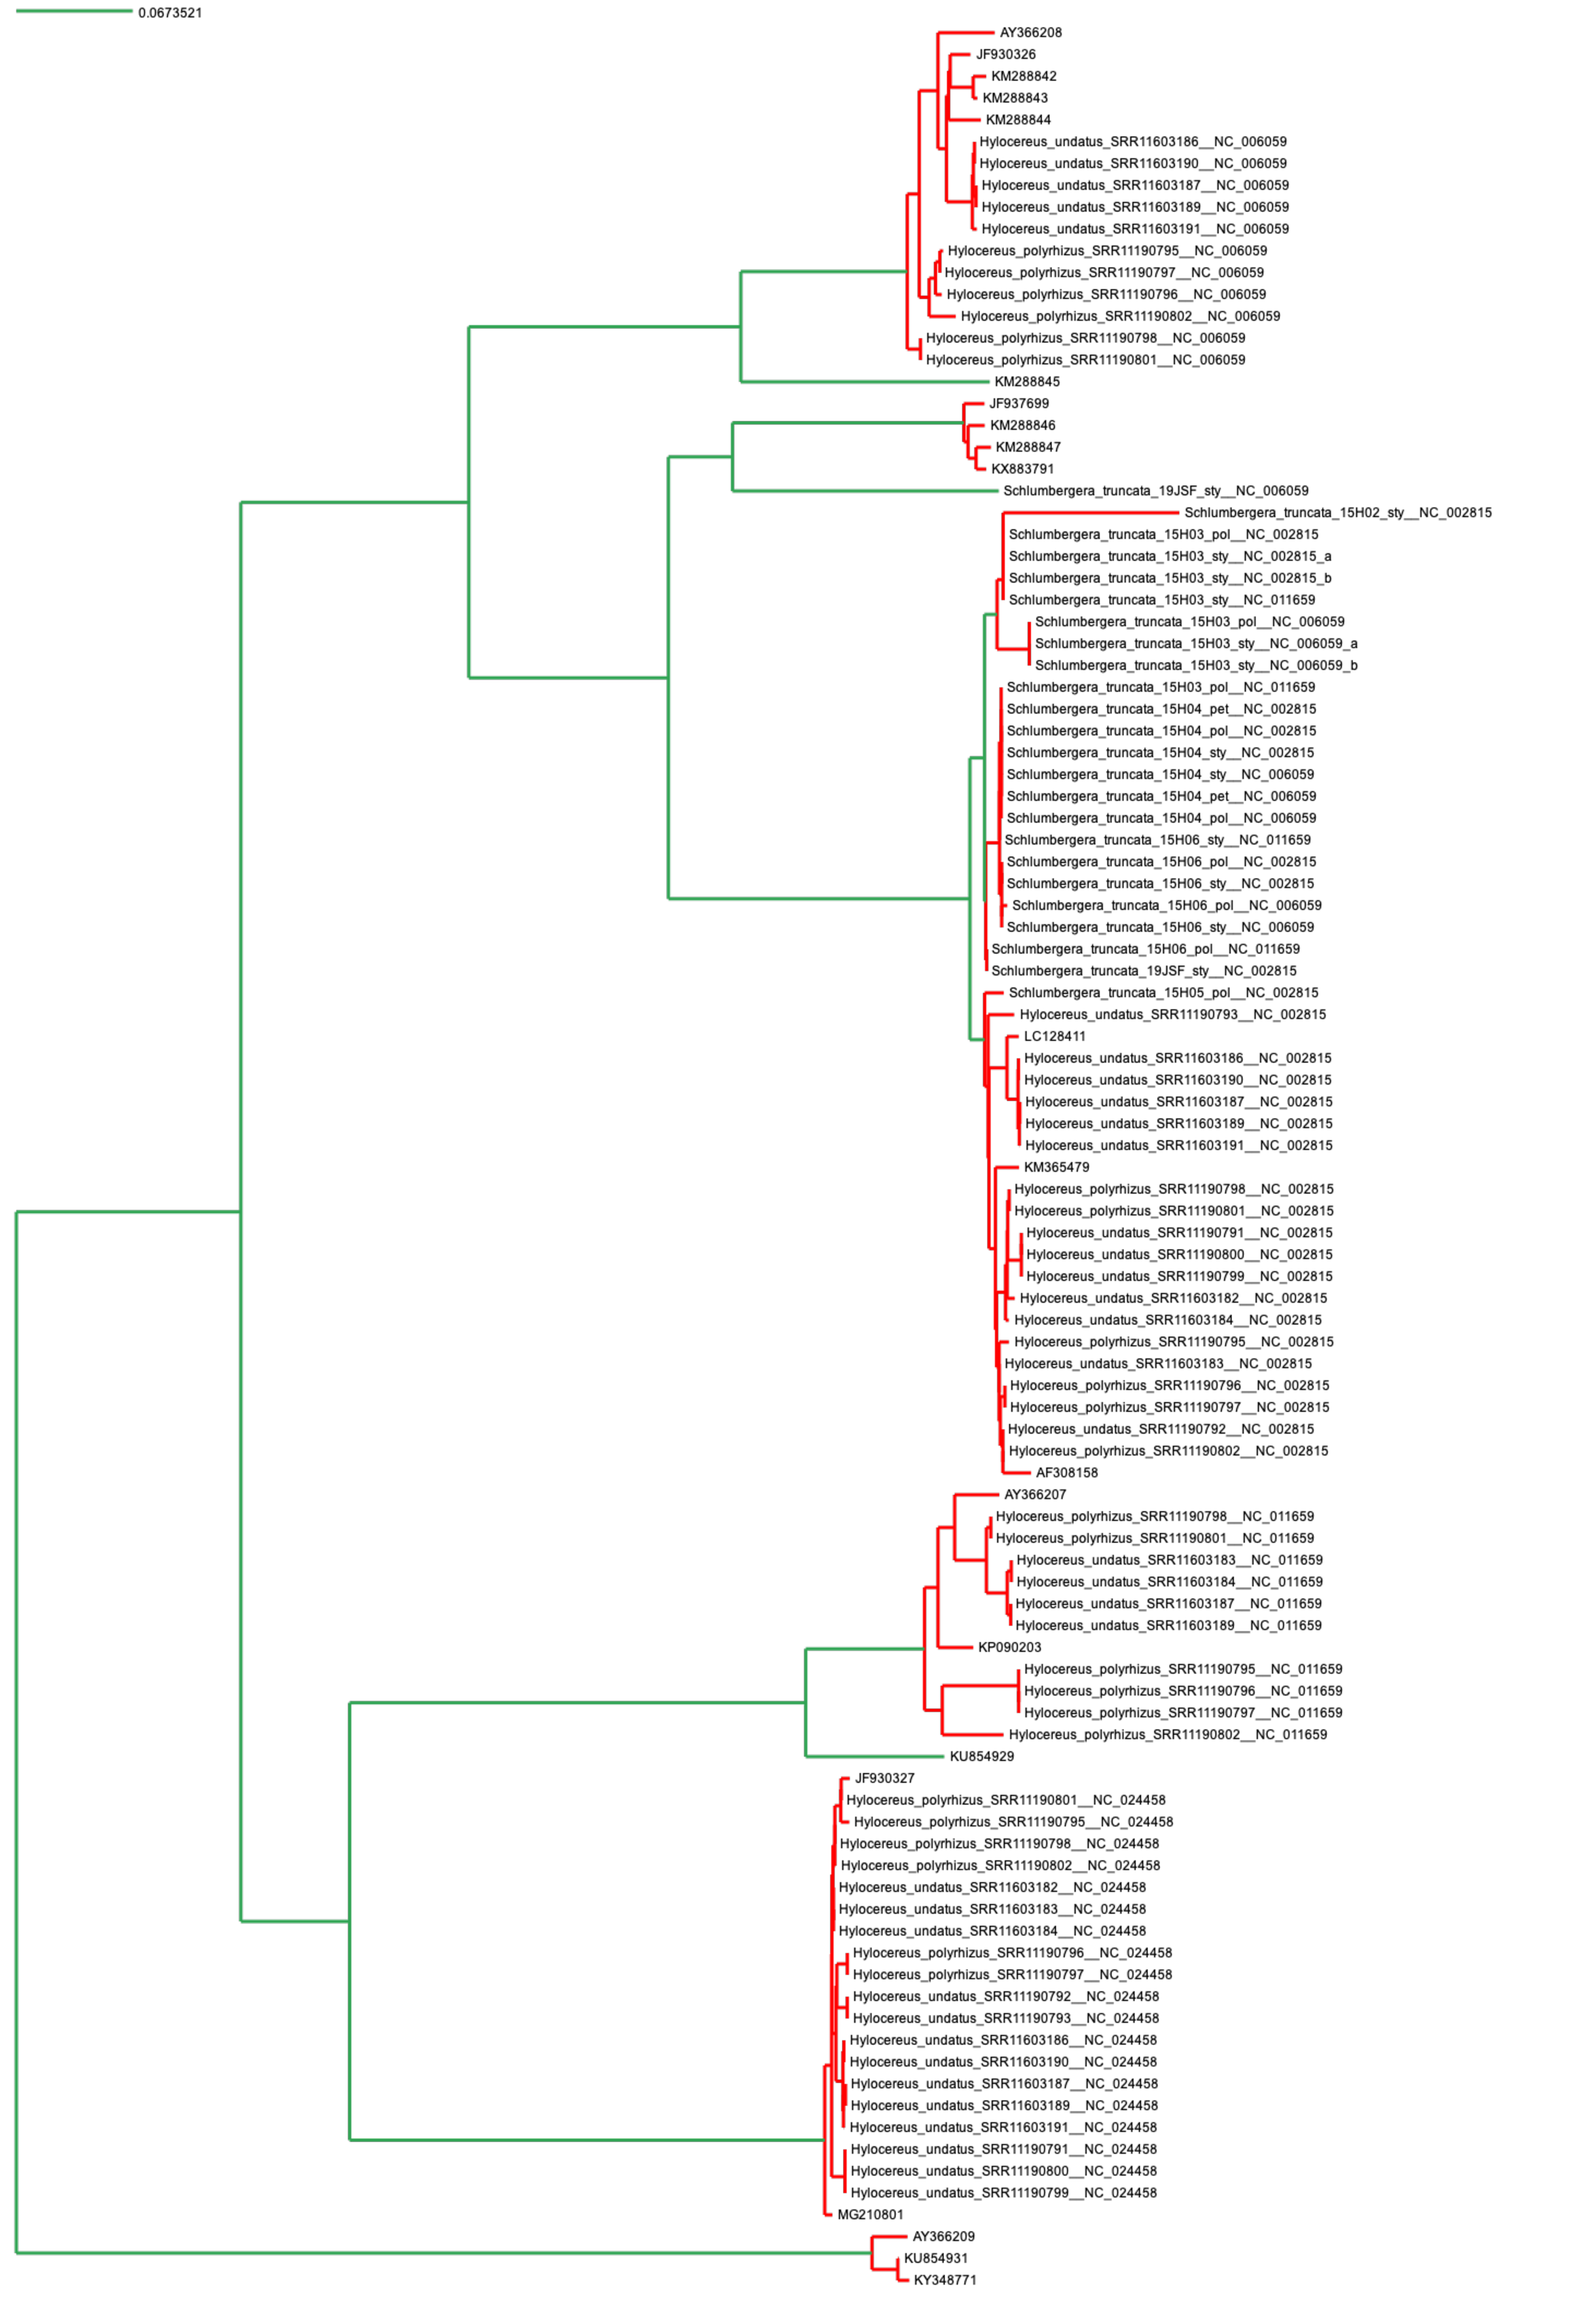
\includegraphics[width=0.8\textwidth]{supplementaryinfo/mptp.pdf}
\label{fig:mptptree}
\end{suppfigure}
\clearpage

%Fig S7:  bPTP tree
\begin{suppfigure}
\centering
\caption{
bPTP whole genome tree with delimitation represented by blue and red coloration. Numbers on nodes represent the posterior probability of the delimitation.
}
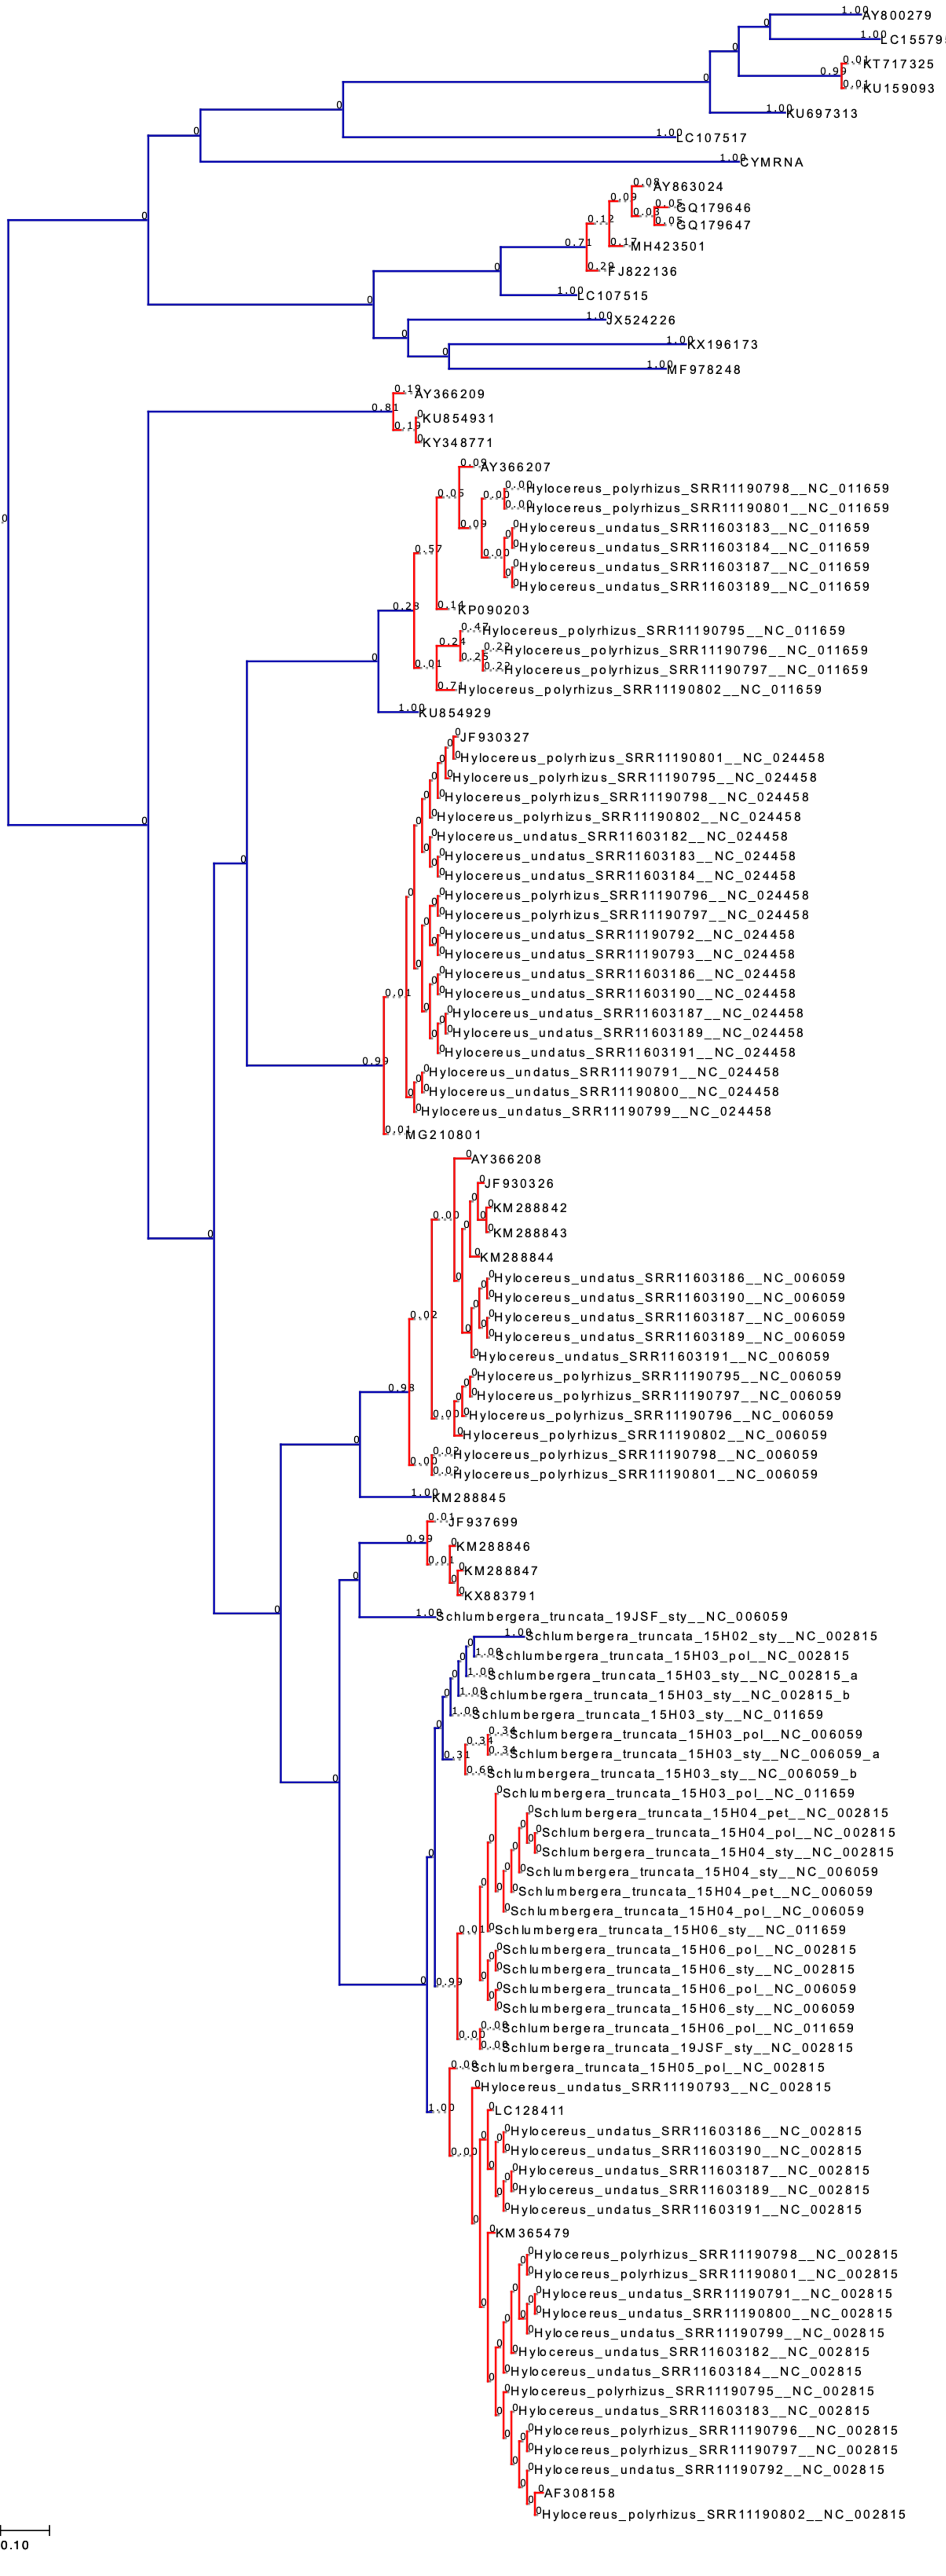
\includegraphics[width=0.4\textwidth]{supplementaryinfo/bptp.pdf}
\label{fig:bptptree}
\end{suppfigure}
\clearpage




%Fig S13: RDRP heatmap
\begin{suppfigure}
\centering
\caption{
Heatmap displaying sequence similarity for aligned ORF1 gene RdRp (RNA-dependent RNA polymerase), which is the largest gene in the potexvirus genome. The genes (n=95) were extracted from each assembled sequence and aligned with MAFFT v7.490. Sequence similarity percentage was calculated across the 5268 nt aligned sequences in \textit{R} using the \textit{dist.dna} function from ape v. 5.7-1. Darker squares represent areas of higher percentage similarity, and values below the ICTV-suggested 72 percent nt identity are represented in a lighter yellow green.
}
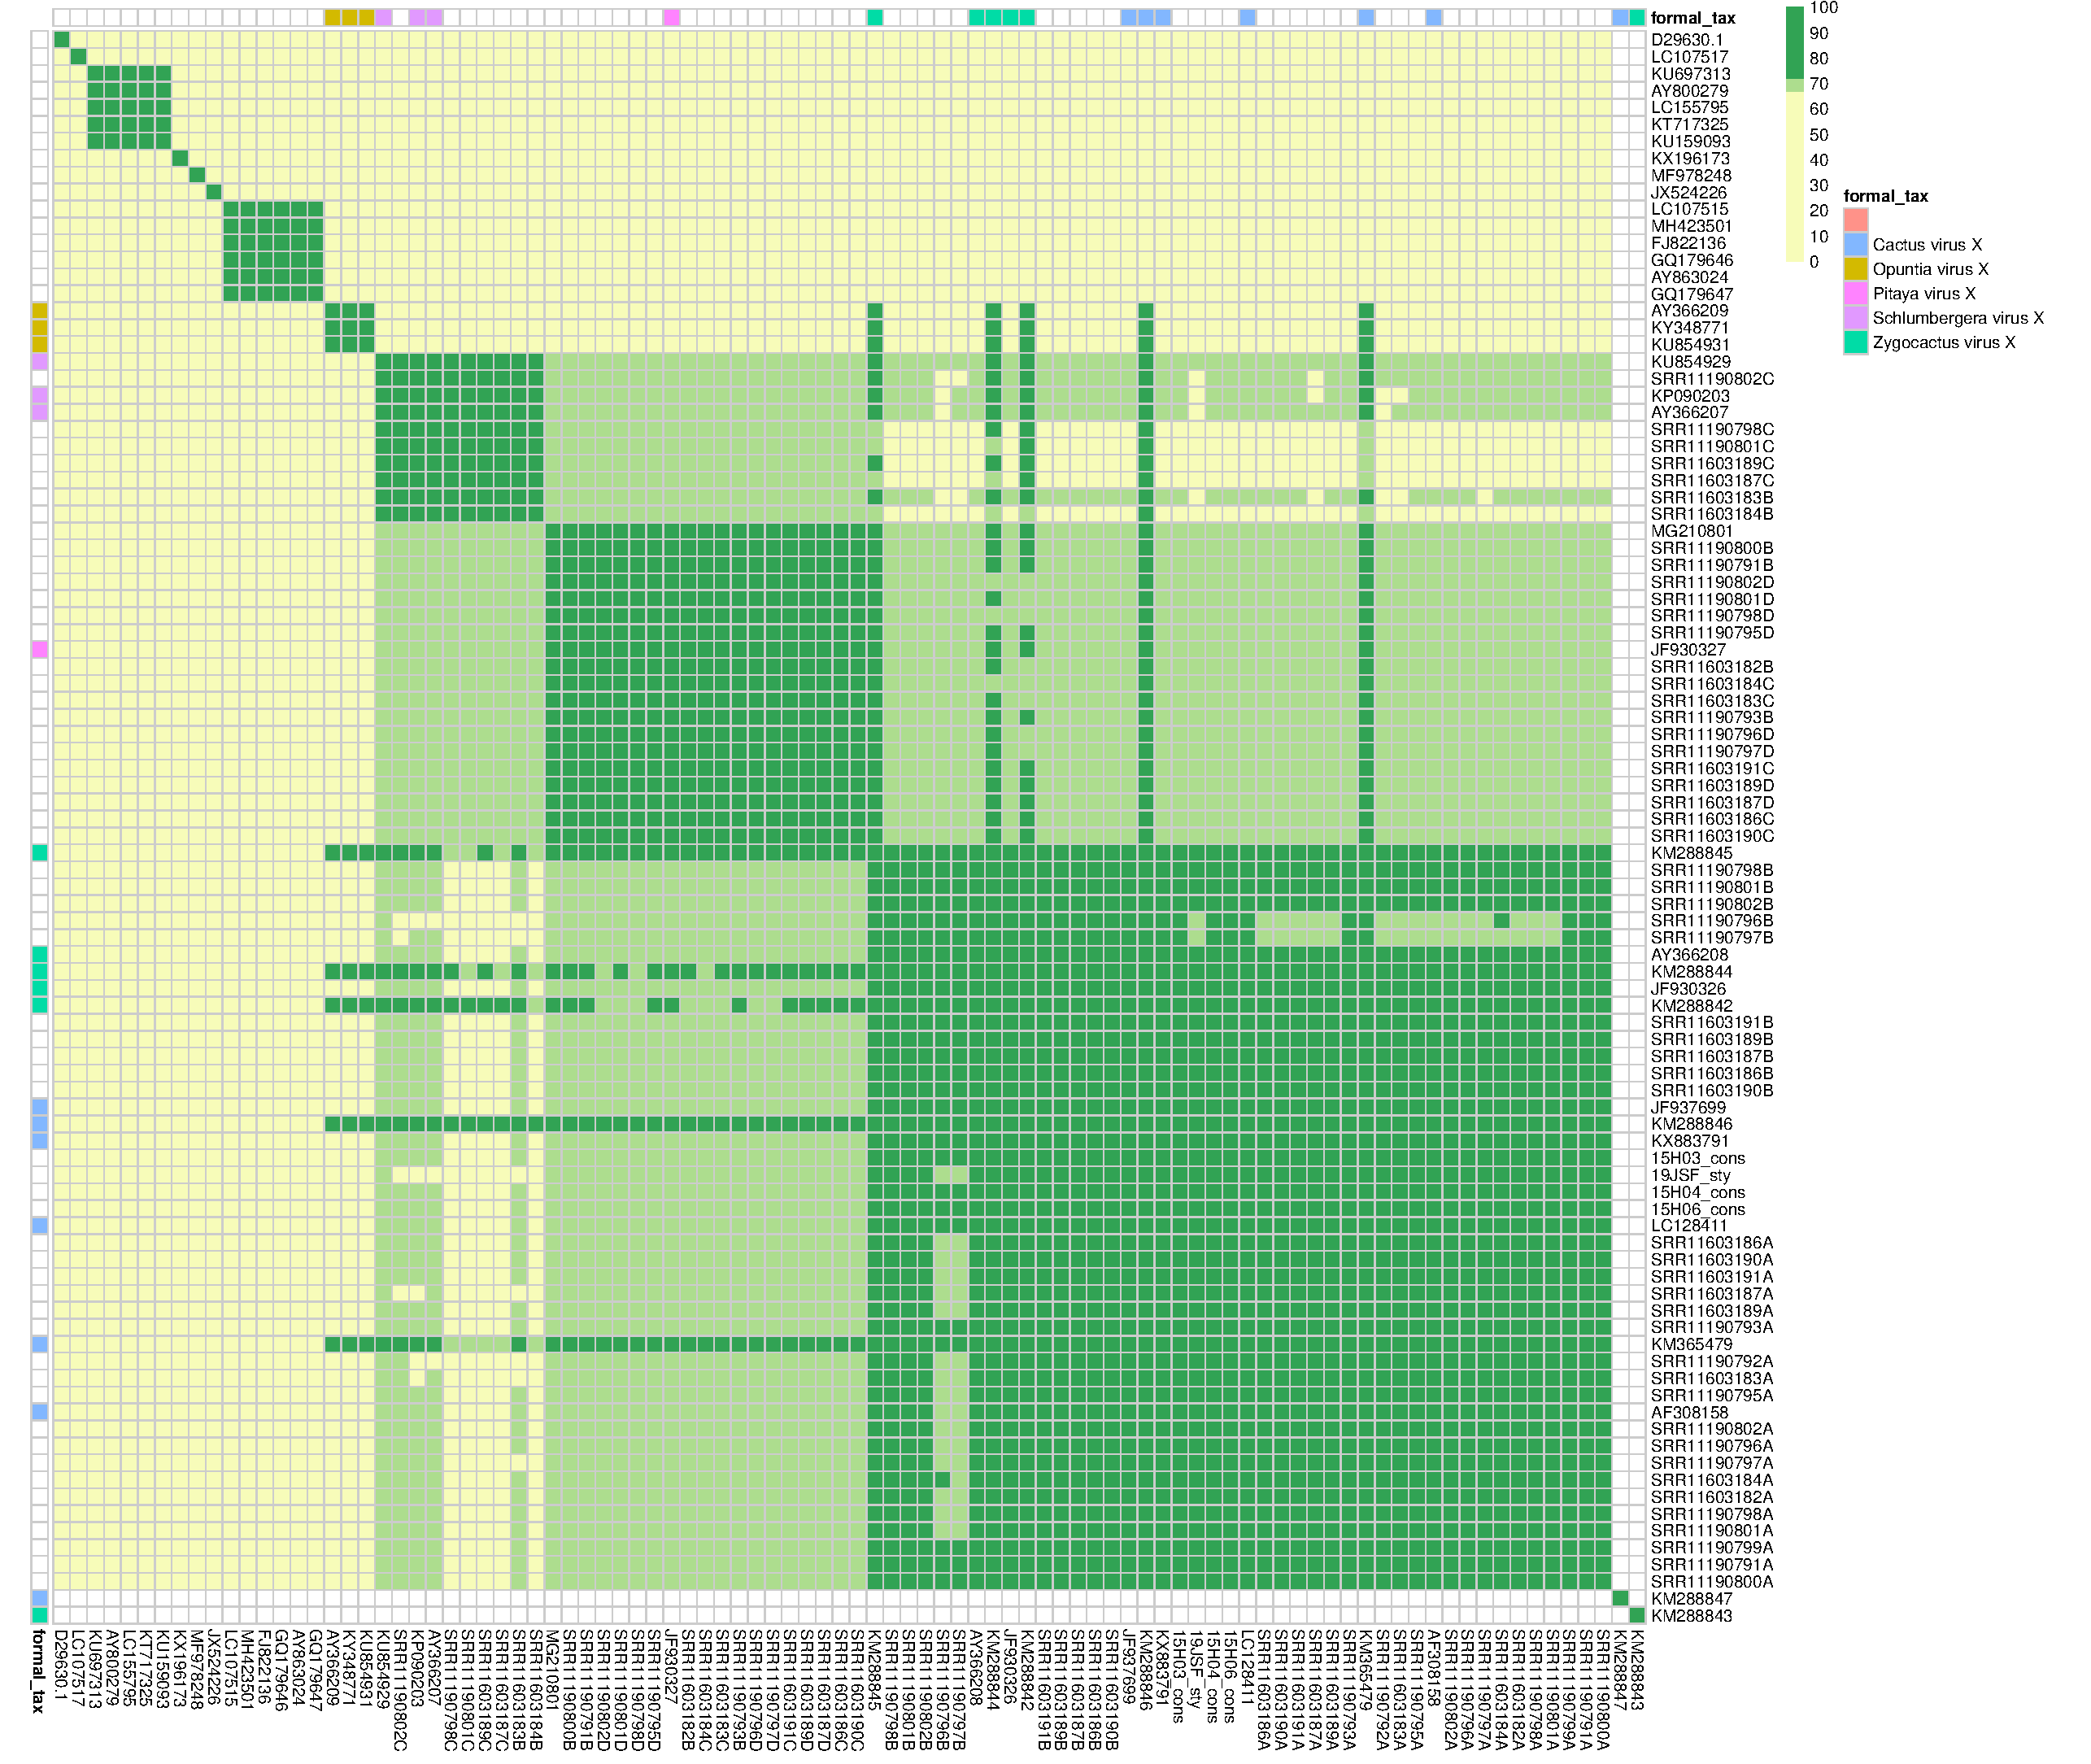
\includegraphics[width=1\textwidth]{figures/heatmap_rdrp.pdf}
\label{fig:heat}
\end{suppfigure}
\clearpage

%Fig S13: CP heatmap
\begin{suppfigure}
\centering
\caption{
Heatmap displaying sequence similarity for Coat Protein (CP) sequences, using the same coloration as above. CP in potexviruses is typically located in ORF5 and this alignment represents 93 sequences each 714 nt in length.
}
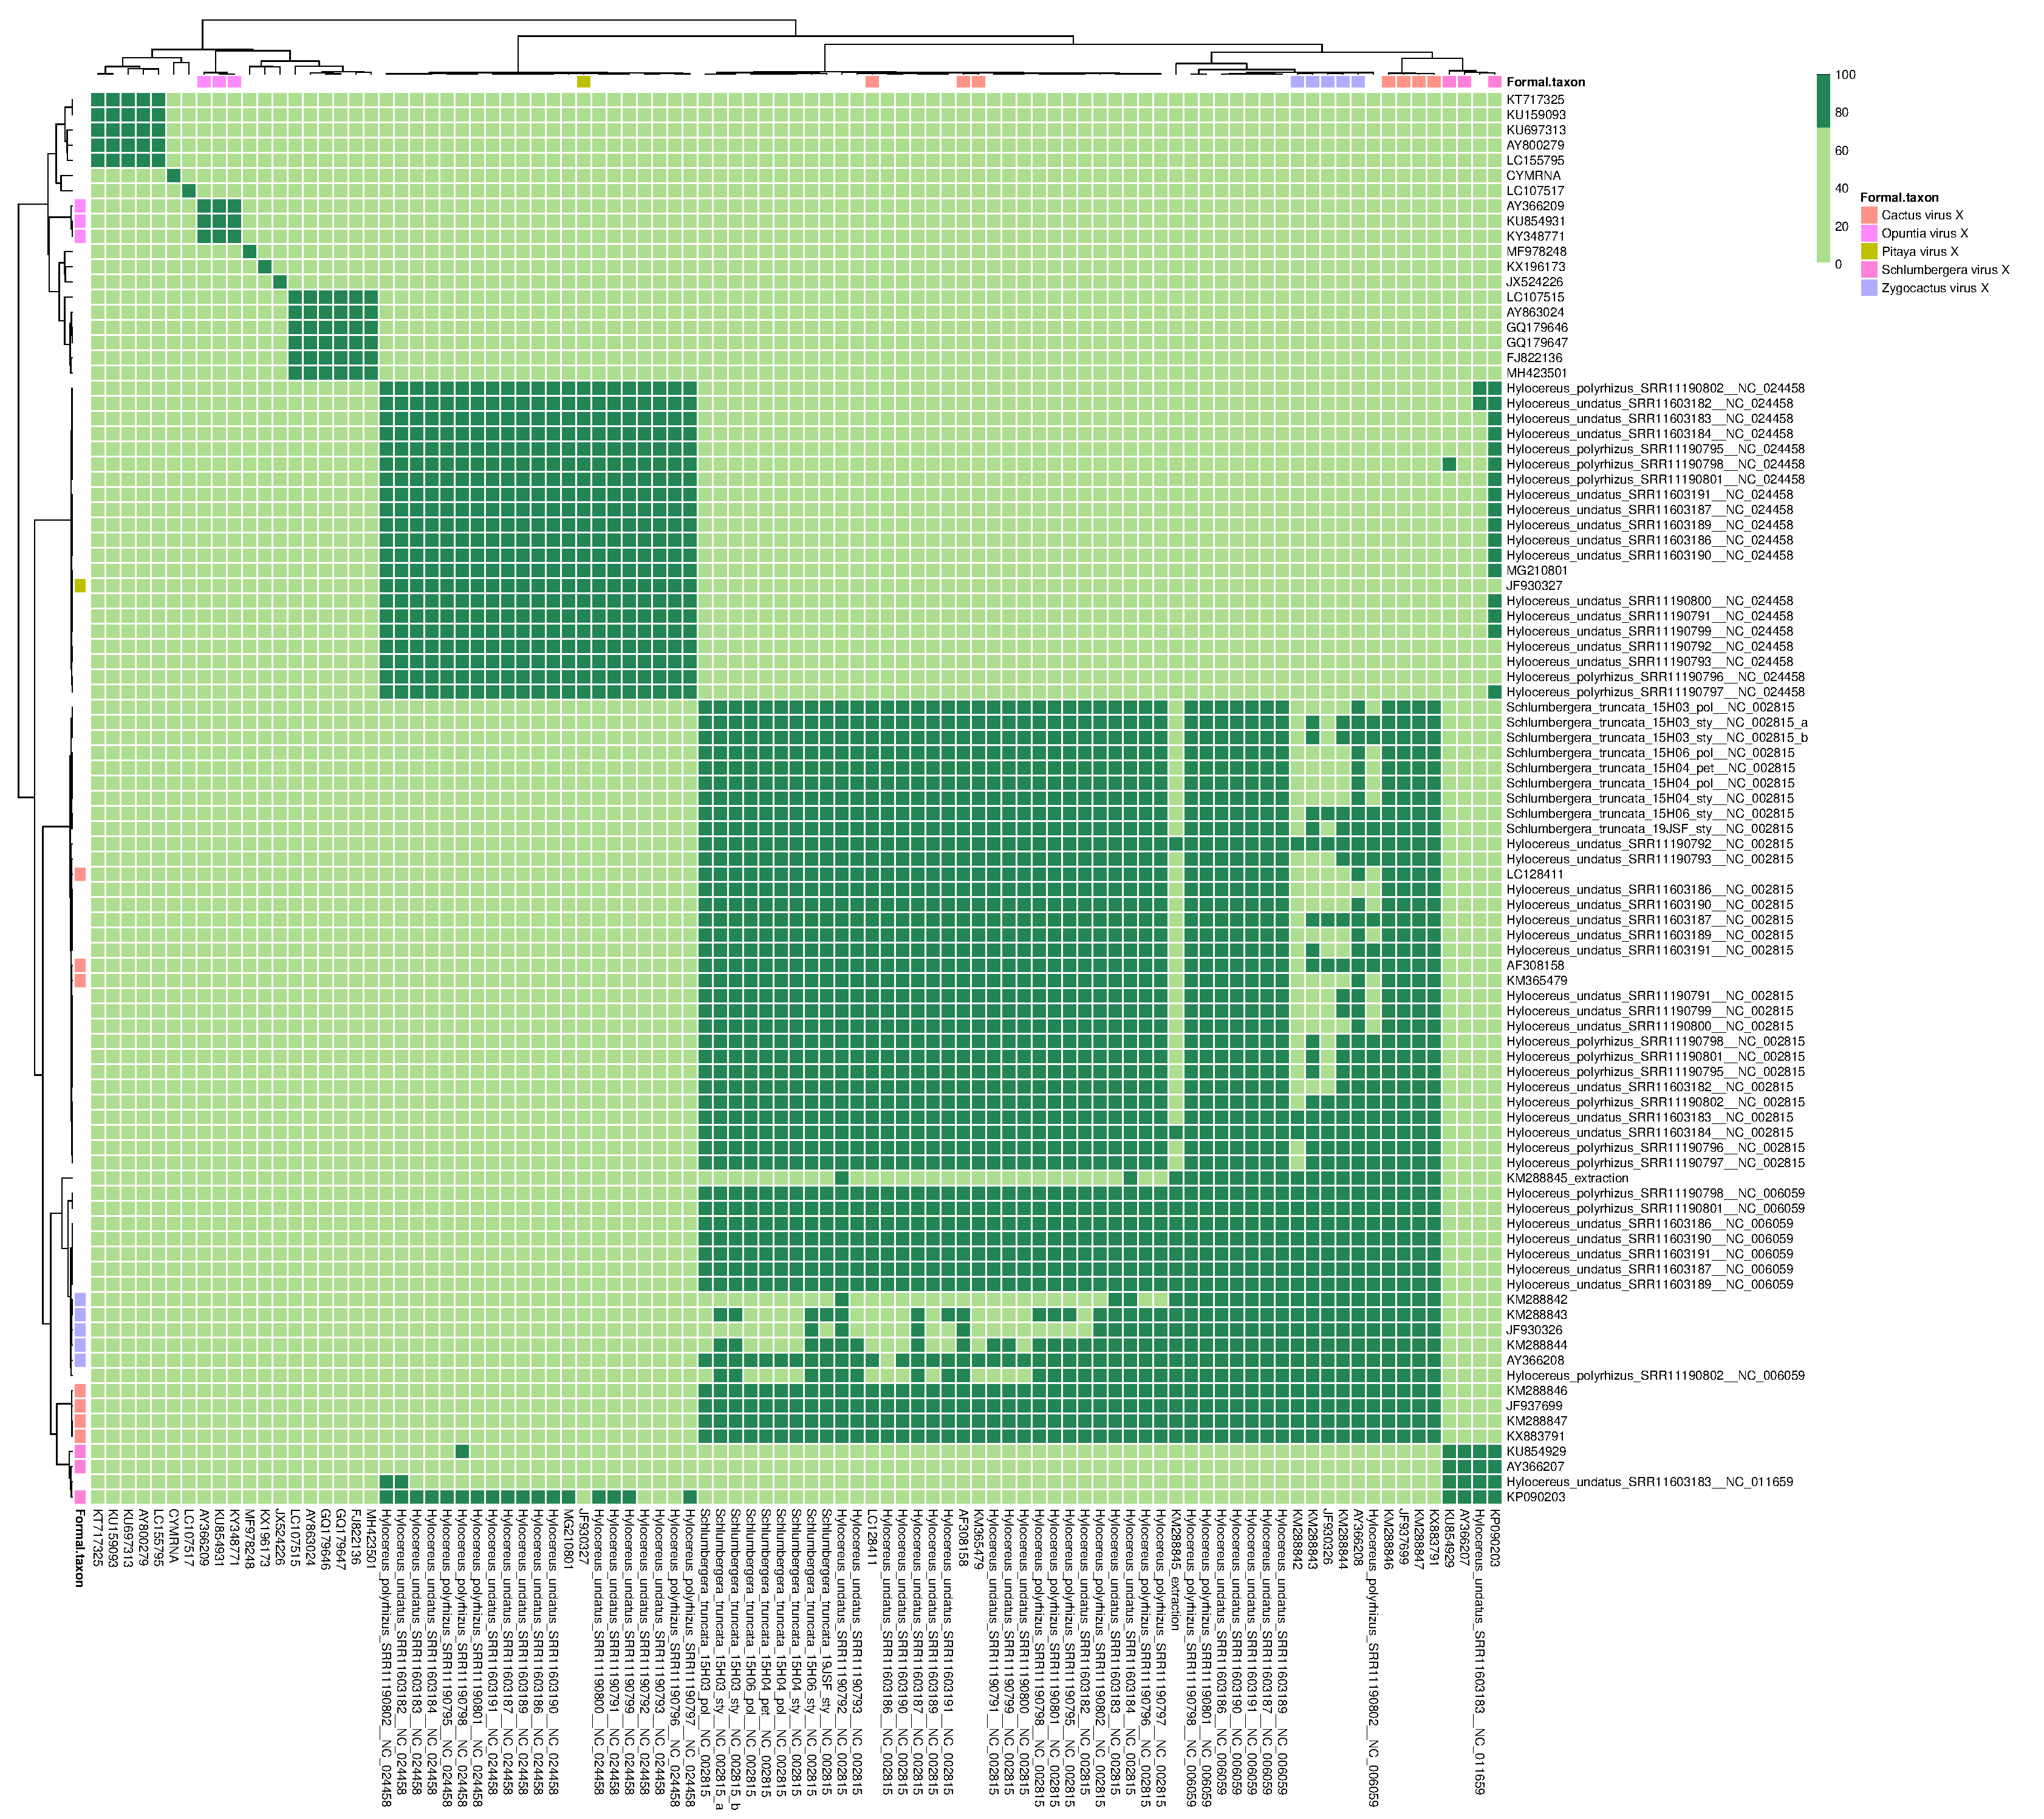
\includegraphics[width=1\textwidth]{figures/heatmap_cp.pdf}
\label{fig:heatmapcp}
\end{suppfigure}
\clearpage
 


%
% TABLES https://www.tablesgenerator.com/
%Table S1: RNA-seq and assembly stats

% Please add the following required packages to your document preamble:
% \usepackage{graphicx}
\clearpage
\newgeometry{landscape}
\begin{supptable}[ht]
\caption{
Genomes and gene sequences downloaded from the NCBI GenBank genome browser, descriptions of the genome, and associated hosts. }
\resizebox{\textwidth}{!}{%
\begin{tabular}{llllll}
Name     & Accession  & Description                                                                                                                                                                                                                                                      & Organism                       & Sequence Length & host                                  \\
AF308158 & AF308158.2 & Cactus virus X, complete genome                                                                                                                                                                                                                                  & Cactus virus X                 & 6614            & Hylocereus undatus                    \\
AY366207 & AY366207.2 & Schlumbergera virus X strain K11, complete genome                                                                                                                                                                                                                & Schlumbergera virus X          & 6633            &                                       \\
AY366208 & AY366208.1 & Zygocactus virus X strain B1 replication-associated protein, triple gene block protein 1, triple gene block protein 2, triple gene block protein 3, and coat protein genes, complete cds                                                                         & Zygocactus virus X             & 6624            &                                       \\
AY366209 & AY366209.1 & Opuntia virus X strain CC10 replication-associated protein, triple gene block protein 1, triple gene block protein 2, triple gene block protein 3, and coat protein genes, complete cds                                                                          & Opuntia virus X                & 6653            &                                       \\
AY800279 & AY800279.1 & Nandina mosaic virus isolate PLH 1, complete genome                                                                                                                                                                                                              & Nandina mosaic virus           & 6066            &                                       \\
AY863024 & AY863024.1 & Alternanthera mosaic virus, complete genome                                                                                                                                                                                                                      & Alternanthera mosaic virus     & 6607            & Phlox stolonifera cv. Sherwood Purple \\
CYMRNA   & D29630.1   & Clover yellow mosaic virus genomic RNA, complete sequence                                                                                                                                                                                                        & Clover yellow mosaic virus     & 7015            &                                       \\
FJ822136 & FJ822136.1 & Alternanthera mosaic virus from Portulaca grandiflora, complete genome                                                                                                                                                                                           & Alternanthera mosaic virus     & 6606            & Portulaca grandiflora                 \\
GQ179646 & GQ179646.1 & Alternanthera mosaic virus isolate SP 3-1, complete genome                                                                                                                                                                                                       & Alternanthera mosaic virus     & 6607            & Phlox stolonifera cv. Sherwood Purple \\
GQ179647 & GQ179647.1 & Alternanthera mosaic virus isolate SP 4-7, complete genome                                                                                                                                                                                                       & Alternanthera mosaic virus     & 6607            & Phlox stolonifera cv. Sherwood Purple \\
JF930326 & JF930326.1 & Zygocactus virus X isolate P39, complete genome                                                                                                                                                                                                                  & Zygocactus virus X             & 6624            & Hylocereus sp.                        \\
JF930327 & JF930327.1 & Pitaya virus X isolate P37, complete genome                                                                                                                                                                                                                      & Pitaya virus X                 & 6677            & Hylocereus sp.                        \\
JF937699 & JF937699.1 & Cactus virus X isolate NTU, complete genome                                                                                                                                                                                                                      & Cactus virus X                 & 6627            & Hylocereus sp.                        \\
JX524226 & JX524226.1 & Papaya mosaic virus isolate PMV-HN, complete genome                                                                                                                                                                                                              & Papaya mosaic virus            & 6656            & Carica papaya                         \\
KM288842 & KM288842.1 & Zygocactus virus X isolate TW-4XB-2 replication-associated protein (RdRP) gene, partial cds; and triple gene block protein 1 (TGB1), triple gene block protein 2 (TGB2), triple gene block protein 3 (TGB3), and coat protein (CP) genes, complete cds           & Zygocactus virus X             & 2403            & Hylocereus sp. (pitaya)               \\
KM288843 & KM288843.1 & Zygocactus virus X isolate TW-456Y-4 triple gene block protein 1 (TGB1) gene, partial cds; and triple gene block protein 2 (TGB2), triple gene block protein 3 (TGB3), and coat protein (CP) genes, complete cds                                                 & Zygocactus virus X             & 1671            & Hylocereus sp. (pitaya)               \\
KM288844 & KM288844.1 & Zygocactus virus X isolate TW-5149-5 replication-associated protein (RdRP) gene, partial cds; and triple gene block protein 1 (TGB1), triple gene block protein 2 (TGB2), triple gene block protein 3 (TGB3), and coat protein (CP) genes, complete cds          & Zygocactus virus X             & 2399            & Hylocereus sp. (pitaya)               \\
KM288845 & KM288845.1 & Zygocactus virus X isolate TW-5149-17 replication-associated protein (RdRP) gene, partial cds; and triple gene block protein 1 (TGB1), triple gene block protein 2 (TGB2), triple gene block protein 3 (TGB3), and coat protein (CP) genes, complete cds         & Zygocactus virus X             & 2397            & Hylocereus sp. (pitaya)               \\
KM288846 & KM288846.1 & Cactus virus X isolate TW-5XB-1 replication-associated protein (RdRP) gene, partial cds; and triple gene block protein 1 (TGB1), triple gene block protein 2 (TGB2), triple gene block protein 3 (TGB3), and coat protein (CP) genes, complete cds               & Cactus virus X                 & 2418            & Hylocereus sp. (pitaya)               \\
KM288847 & KM288847.1 & Cactus virus X isolate TW-456Y-1 triple gene block protein 1 (TGB1) gene, partial cds; and triple gene block protein 2 (TGB2), triple gene block protein 3 (TGB3), and coat protein (CP) genes, complete cds                                                     & Cactus virus X                 & 1675            & Hylocereus sp. (pitaya)               \\
KM365479 & KM365479.1 & Cactus virus X isolate TW-5149-20 replication-associated protein (CVXgp1) gene, partial cds; and triple gene block protein 1 (CVXgp2), triple gene block protein 2 (CVXgp3), triple gene block protein 3 (CVXgp4), and coat protein (CVXgp5) genes, complete cds & Cactus virus X                 & 2396            & Hylocereus sp. (pitaya)               \\
KP090203 & KP090203.1 & Schlumbergera virus X isolate Palma-PE, complete genome                                                                                                                                                                                                          & Schlumbergera virus X          & 6615            & Opuntia cochenillifera                \\
KT717325 & KT717325.1 & Plantago asiatica mosaic virus isolate kr, complete genome                                                                                                                                                                                                       & Plantago asiatica mosaic virus & 6101            & Lilium sp.                            \\
KU159093 & KU159093.1 & Plantago asiatica mosaic virus isolate Ko-YS, complete genome                                                                                                                                                                                                    & Plantago asiatica mosaic virus & 6102            & lily                                  \\
KU697313 & KU697313.1 & Plantago asiatica mosaic virus isolate Gunwi, complete genome                                                                                                                                                                                                    & Plantago asiatica mosaic virus & 6130            & Plantago asiatica                     \\
KU854929 & KU854929.1 & Schlumbergera virus X isolate nopal verdura 1, complete genome                                                                                                                                                                                                   & Schlumbergera virus X          & 6646            & Opuntia ficus-indica                  \\
KU854931 & KU854931.1 & Opuntia virus X isolate nopal verdura-1, complete genome                                                                                                                                                                                                         & Opuntia virus X                & 6667            & Opuntia ficus-indica                  \\
KX196173 & KX196173.2 & Senna mosaic virus isolate Brazilian, complete genome                                                                                                                                                                                                            & Senna mosaic virus             & 6775            & Senna occidentalis                    \\
KX883791 & KX883791.1 & Cactus virus X strain SCM51431 ORF1, ORF2, ORF3, and ORF4 genes, complete cds                                                                                                                                                                                    & Cactus virus X                 & 6610            & Diptera                               \\
KY348771 & KY348771.1 & Opuntia virus X isolate Noptuna-Mex, complete genome                                                                                                                                                                                                             & Opuntia virus X                & 6656            & Opuntia albicarpa cv. nopal tunero    \\
LC107515 & LC107515.1 & Alternanthera mosaic virus genomic RNA, complete genome, isolate: Ac                                                                                                                                                                                             & Alternanthera mosaic virus     & 6604            & Achyranthes bidentata                 \\
LC107517 & LC107517.1 & Hydrangea ringspot virus genomic RNA, complete genome, isolate: Gu2                                                                                                                                                                                              & Hydrangea ringspot virus       & 6196            & Hydrangea macrophylla                 \\
LC128411 & LC128411.1 & Cactus virus X genomic RNA, complete genome                                                                                                                                                                                                                      & Cactus virus X                 & 6618            & Hylocereus undatus                    \\
LC155795 & LC155795.1 & Plantago asiatica mosaic virus genomic RNA, complete genome, isolate: NJ                                                                                                                                                                                         & Plantago asiatica mosaic virus & 6122            & Nandina domestica                     \\
MF978248 & MF978248.1 & Babaco mosaic virus isolate Tandapi, complete genome                                                                                                                                                                                                             & Babaco mosaic virus            & 6692            & Vasconcellea x heilbornii             \\
MG210801 & MG210801.1 & Mytcor virus 1 replicative protein gene, partial cds; and protein 2 and protein 3 genes, complete cds                                                                                                                                                            & Mytcor virus 1                 & 5689            & Mytilus coruscus                      \\
MH423501 & MH423501.1 & Alternanthera mosaic virus isolate DH, complete genome                                                                                                                                                                                                           & Alternanthera mosaic virus     & 6598            & Epiphyllum sp. cv. Dragon Heart      
\end{tabular}%
}
\end{supptable}
\restoregeometry
\clearpage


\begin{supptable}[ht]

\caption{
Newly assembled viral sequences originating from SRA plant datasets.
}% Please add the following required packages to your document preamble:
% \usepackage{graphicx}
\resizebox{\textwidth}{!}{%
\begin{tabular}{lllll}
\hline
Phylogeny\_tipname   & sample\_name & Description\_mapped\_to & Sequence Length & host                  \\ \hline
SRR11190795\_NC2815  & SRR11190795  & NC\_002815              & 6614            & Hylocereus polyrhizus \\
SRR11190795\_NC6059  & SRR11190795  & NC\_006059              & 6624            & Hylocereus polyrhizus \\
SRR11190795\_NC11659 & SRR11190795  & NC\_011659              & 6633            & Hylocereus polyrhizus \\
SRR11190795\_NC24458 & SRR11190795  & NC\_024458              & 6677            & Hylocereus polyrhizus \\
SRR11190796\_NC2815  & SRR11190796  & NC\_002815              & 6614            & Hylocereus polyrhizus \\
SRR11190796\_NC6059  & SRR11190796  & NC\_006059              & 6624            & Hylocereus polyrhizus \\
SRR11190796\_NC11659 & SRR11190796  & NC\_011659              & 6633            & Hylocereus polyrhizus \\
SRR11190796\_NC24458 & SRR11190796  & NC\_024458              & 6677            & Hylocereus polyrhizus \\
SRR11190797\_NC2815  & SRR11190797  & NC\_002815              & 6614            & Hylocereus polyrhizus \\
SRR11190797\_NC6059  & SRR11190797  & NC\_006059              & 6624            & Hylocereus polyrhizus \\
SRR11190797\_NC11659 & SRR11190797  & NC\_011659              & 6633            & Hylocereus polyrhizus \\
SRR11190797\_NC24458 & SRR11190797  & NC\_024458              & 6677            & Hylocereus polyrhizus \\
SRR11190798\_NC2815  & SRR11190798  & NC\_002815              & 6614            & Hylocereus polyrhizus \\
SRR11190798\_NC6059  & SRR11190798  & NC\_006059              & 6624            & Hylocereus polyrhizus \\
SRR11190798\_NC11659 & SRR11190798  & NC\_011659              & 6633            & Hylocereus polyrhizus \\
SRR11190798\_NC24458 & SRR11190798  & NC\_024458              & 6677            & Hylocereus polyrhizus \\
SRR11190801\_NC2815  & SRR11190801  & NC\_002815              & 6614            & Hylocereus polyrhizus \\
SRR11190801\_NC6059  & SRR11190801  & NC\_006059              & 6624            & Hylocereus polyrhizus \\
SRR11190801\_NC11659 & SRR11190801  & NC\_011659              & 6633            & Hylocereus polyrhizus \\
SRR11190801\_NC24458 & SRR11190801  & NC\_024458              & 6677            & Hylocereus polyrhizus \\
SRR11190802\_NC2815  & SRR11190802  & NC\_002815              & 6614            & Hylocereus polyrhizus \\
SRR11190802\_NC6059  & SRR11190802  & NC\_006059              & 6624            & Hylocereus polyrhizus \\
SRR11190802\_NC11659 & SRR11190802  & NC\_011659              & 6633            & Hylocereus polyrhizus \\
SRR11190802\_NC24458 & SRR11190802  & NC\_024458              & 6677            & Hylocereus polyrhizus \\
SRR11190791\_NC2815  & SRR11190791  & NC\_002815              & 6614            & Hylocereus undatus    \\
SRR11190791\_NC24458 & SRR11190791  & NC\_024458              & 6677            & Hylocereus undatus    \\
SRR11190792\_NC2815  & SRR11190792  & NC\_002815              & 6614            & Hylocereus undatus    \\
SRR11190792\_NC24458 & SRR11190792  & NC\_024458              & 6677            & Hylocereus undatus    \\
SRR11190793\_NC2815  & SRR11190793  & NC\_002815              & 6614            & Hylocereus undatus    \\
SRR11190793\_NC24458 & SRR11190793  & NC\_024458              & 6677            & Hylocereus undatus    \\
SRR11190799\_NC2815  & SRR11190799  & NC\_002815              & 6614            & Hylocereus undatus    \\
SRR11190799\_NC24458 & SRR11190799  & NC\_024458              & 6677            & Hylocereus undatus    \\
SRR11190800\_NC2815  & SRR11190800  & NC\_002815              & 6614            & Hylocereus undatus    \\
SRR11190800\_NC24458 & SRR11190800  & NC\_024458              & 6677            & Hylocereus undatus    \\
SRR11603182\_NC2815  & SRR11603182  & NC\_002815              & 6614            & Hylocereus undatus    \\
SRR11603182\_NC24458 & SRR11603182  & NC\_024458              & 6677            & Hylocereus undatus    \\
SRR11603183\_NC2815  & SRR11603183  & NC\_002815              & 6614            & Hylocereus undatus    \\
SRR11603183\_NC11659 & SRR11603183  & NC\_011659              & 6633            & Hylocereus undatus    \\
SRR11603183\_NC24458 & SRR11603183  & NC\_024458              & 6677            & Hylocereus undatus    \\
SRR11603184\_NC2815  & SRR11603184  & NC\_002815              & 6614            & Hylocereus undatus    \\
SRR11603184\_NC11659 & SRR11603184  & NC\_011659              & 6633            & Hylocereus undatus    \\
SRR11603184\_NC24458 & SRR11603184  & NC\_024458              & 6677            & Hylocereus undatus    \\
SRR11603186\_NC2815  & SRR11603186  & NC\_002815              & 6614            & Hylocereus undatus    \\
SRR11603186\_NC6059  & SRR11603186  & NC\_006059              & 6624            & Hylocereus undatus    \\
SRR11603186\_NC24458 & SRR11603186  & NC\_024458              & 6677            & Hylocereus undatus    \\
SRR11603187\_NC2815  & SRR11603187  & NC\_002815              & 6614            & Hylocereus undatus    \\
SRR11603187\_NC6059  & SRR11603187  & NC\_006059              & 6624            & Hylocereus undatus    \\
SRR11603187\_NC11659 & SRR11603187  & NC\_011659              & 6633            & Hylocereus undatus    \\
SRR11603187\_NC24458 & SRR11603187  & NC\_024458              & 6677            & Hylocereus undatus    \\
SRR11603189\_NC2815  & SRR11603189  & NC\_002815              & 6614            & Hylocereus undatus    \\
SRR11603189\_NC6059  & SRR11603189  & NC\_006059              & 6624            & Hylocereus undatus    \\
SRR11603189\_NC11659 & SRR11603189  & NC\_011659              & 6633            & Hylocereus undatus    \\
SRR11603189\_NC24458 & SRR11603189  & NC\_024458              & 6677            & Hylocereus undatus    \\
SRR11603190\_NC2815  & SRR11603190  & NC\_002815              & 6614            & Hylocereus undatus    \\
SRR11603190\_NC6059  & SRR11603190  & NC\_006059              & 6624            & Hylocereus undatus    \\
SRR11603190\_NC24458 & SRR11603190  & NC\_024458              & 6677            & Hylocereus undatus    \\
SRR11603191\_NC2815  & SRR11603191  & NC\_002815              & 6614            & Hylocereus undatus    \\
SRR11603191\_NC6059  & SRR11603191  & NC\_006059              & 6624            & Hylocereus undatus    \\
SRR11603191\_NC24458 & SRR11603191  & NC\_024458              & 6677            & Hylocereus undatus    \\ \hline
\end{tabular}%
}
\end{supptable}
\end{document}
